\chapter{Semantic Scaling for Generalizable Video Retrieval}
\label{ch:universal-video-retrieval}

\section{Introduction}

Chapter~\ref{ch:introduction} identifies semantic scaling as the first bottleneck in the retrieval pipeline. A generalizable video representation must support heterogeneous query formats, semantic domains, and relevance granularities rather than specialize in a single benchmark setting. The literature on video embedding models and heterogeneous retrieval evaluation is reviewed centrally in \S\ref{sec:lr-embedding} and \S\ref{sec:lr-benchmarks}.

Current video embedding models are commonly trained on massive datasets with simple and noisy text annotations, such as WebVid~\cite{bain2021frozen}. This practice yields strong results for coarse-grained text-to-video retrieval on standard benchmarks such as MSRVTT~\cite{xu2016msr}, but the resulting models struggle with the complexity of diverse real-world retrieval scenarios~(Figure~\ref{fig:uvr}). First, a narrow semantic distribution renders these models less effective in fine-grained queries required to understand spatial relations or temporal dynamics~\cite{xu2025carebench}, as well as in long-context retrieval within lengthy videos~\cite{cai2025lovr}. Second, the scope of applicable tasks is restricted, with limited support for diverse query formats, such as composed retrieval using text-and-image pairs. Furthermore, these capability gaps are often obscured by the fragmented evaluation landscape, where models are optimized and tested on isolated benchmarks, preventing a clear understanding of comprehensive generalization.

\begin{figure}[t]
    \centering
    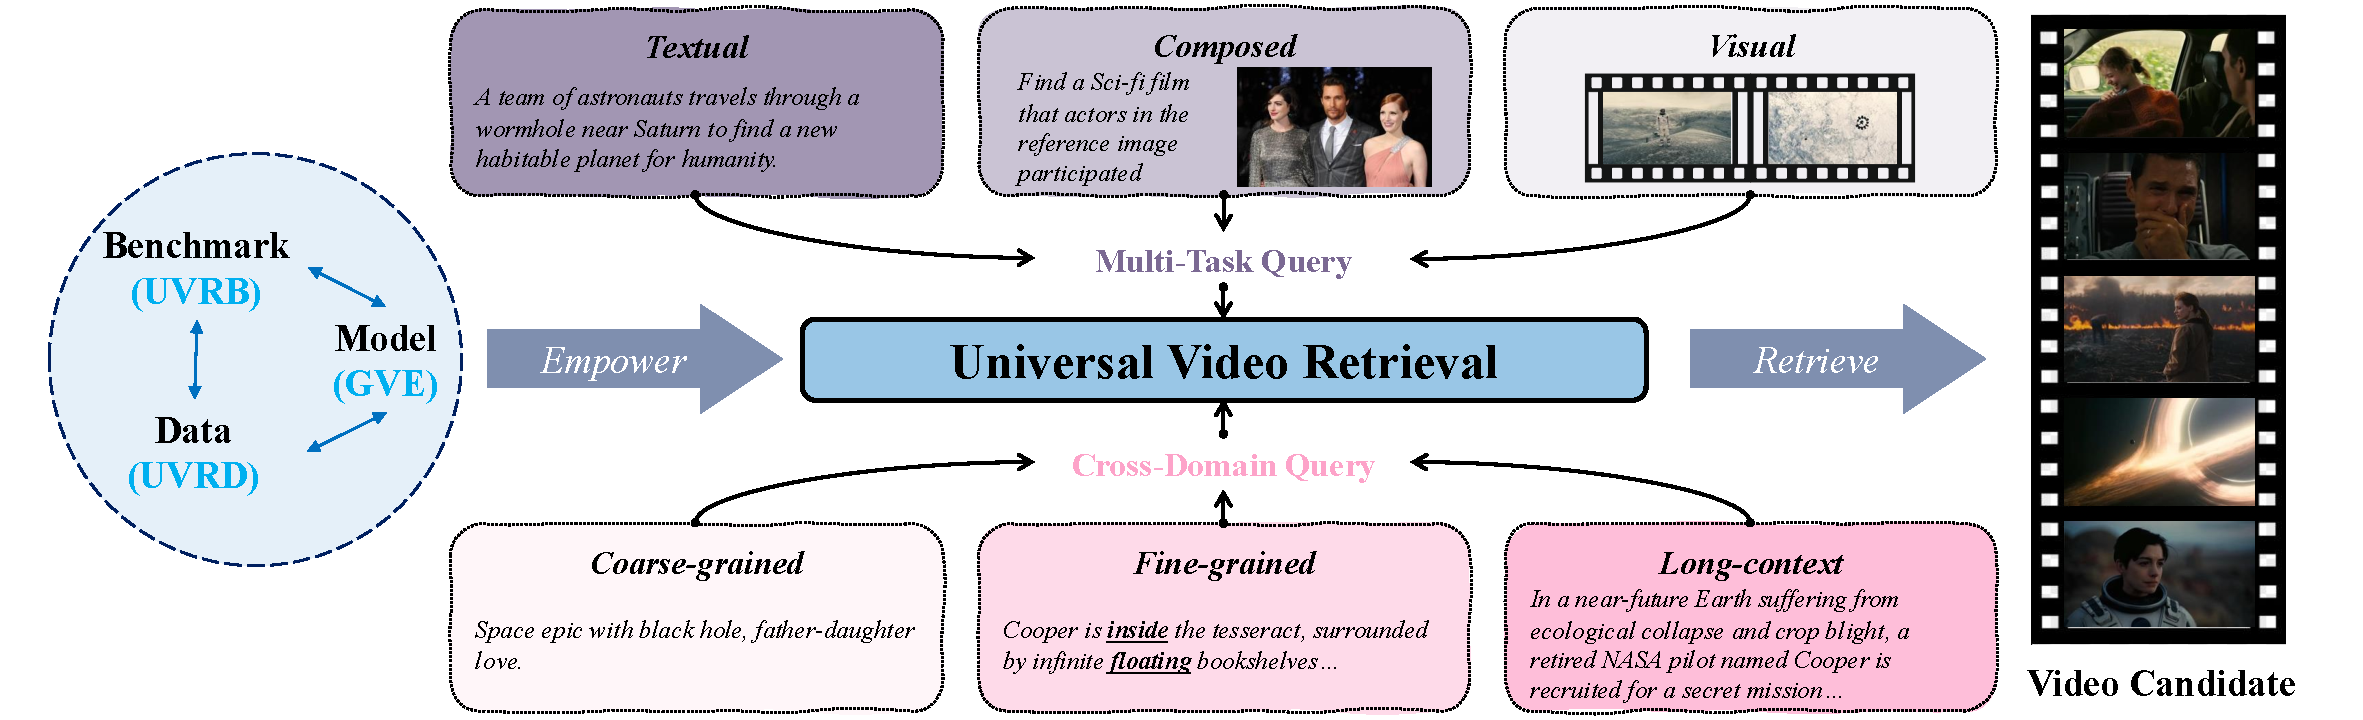
\includegraphics[width=\linewidth]{uvr.pdf}
    \caption{Universal Video Retrieval organizes heterogeneous retrieval settings into a unified capability space.}
    \label{fig:uvr}
\end{figure}

Therefore, to establish a framework for universal video retrieval that supports multi-domain, multi-granularity, and multi-task capabilities, \textit{two critical hurdles in data and modeling} must be addressed:  
(1)~\textit{Large-Scale Quality-Controlled Data Synthesis}: Existing datasets are either too small or are biased, while collecting a new, massive dataset is prohibitively expensive. Growing works attempt to synthesize data to address this challenge~\cite{chen2023vast,chai2024auroracap,ventura2024covr}. However, these resources often exhibit uneven quality and distribution. Therefore, gaining precise control over the properties of large-scale, cross-domain, multi-task data via a unified synthesis process is a primary challenge.  
(2)~\textit{Interconnected Multi-task Representation Learning}: A critical, often-ignored aspect is the inherent hierarchy among tasks. Foundational abilities such as spatial perception (e.g., object recognition) serve as building blocks for higher-order temporal reasoning (e.g., action recognition). This principle is evidenced by the remarkable success of image-only trained models like GME~\cite{Zhang_2025_CVPR} on video retrieval tasks (see Figure~\ref{gve:fig:radar_uvrb}), highlighting latent cross-task adaptability. Nevertheless, conventional models that assume task independence fail to capitalize on this structure, which is a key to unlocking superior generalization.

To this end, we propose a holistic framework that couples targeted data synthesis with stable modeling.  
First, to expose the concrete limitations of current approaches, we perform a standardized evaluation across $16$ established public datasets, assessing $14$ state-of-the-art models under unified preprocessing and metrics.  
Second, directly guided by the capability gaps identified in this evaluation (e.g., deficiencies in temporal and composed retrieval), we design \textbf{V-SynFlow}. This workflow transforms raw videos into a targeted, high-quality dataset, the \textbf{Universal Video Retrieval Dataset~(UVRD)}, consisting of over $1.55$ million multi-task pairs.  
Third, to ensure stability during heterogeneous training, we apply the \textbf{Modality Pyramid}, a training curriculum that leverages inherent task dependencies. It optimizes the \textbf{General Video Embedder (GVE)} by prioritizing foundational tasks before progressing to complex ones, facilitating smooth gradient convergence.

Extensive experiments validate the effectiveness of the GVE model~(Figure~\ref{gve:fig:radar_uvrb}). In addition to strong zero-shot performance, the analysis reveals that performance on conventional benchmarks correlates poorly with overall retrieval capability; meanwhile, partially relevant video retrieval can serve as a representative indicator of universal video retrieval.

\begin{figure}[t]
   \centering
   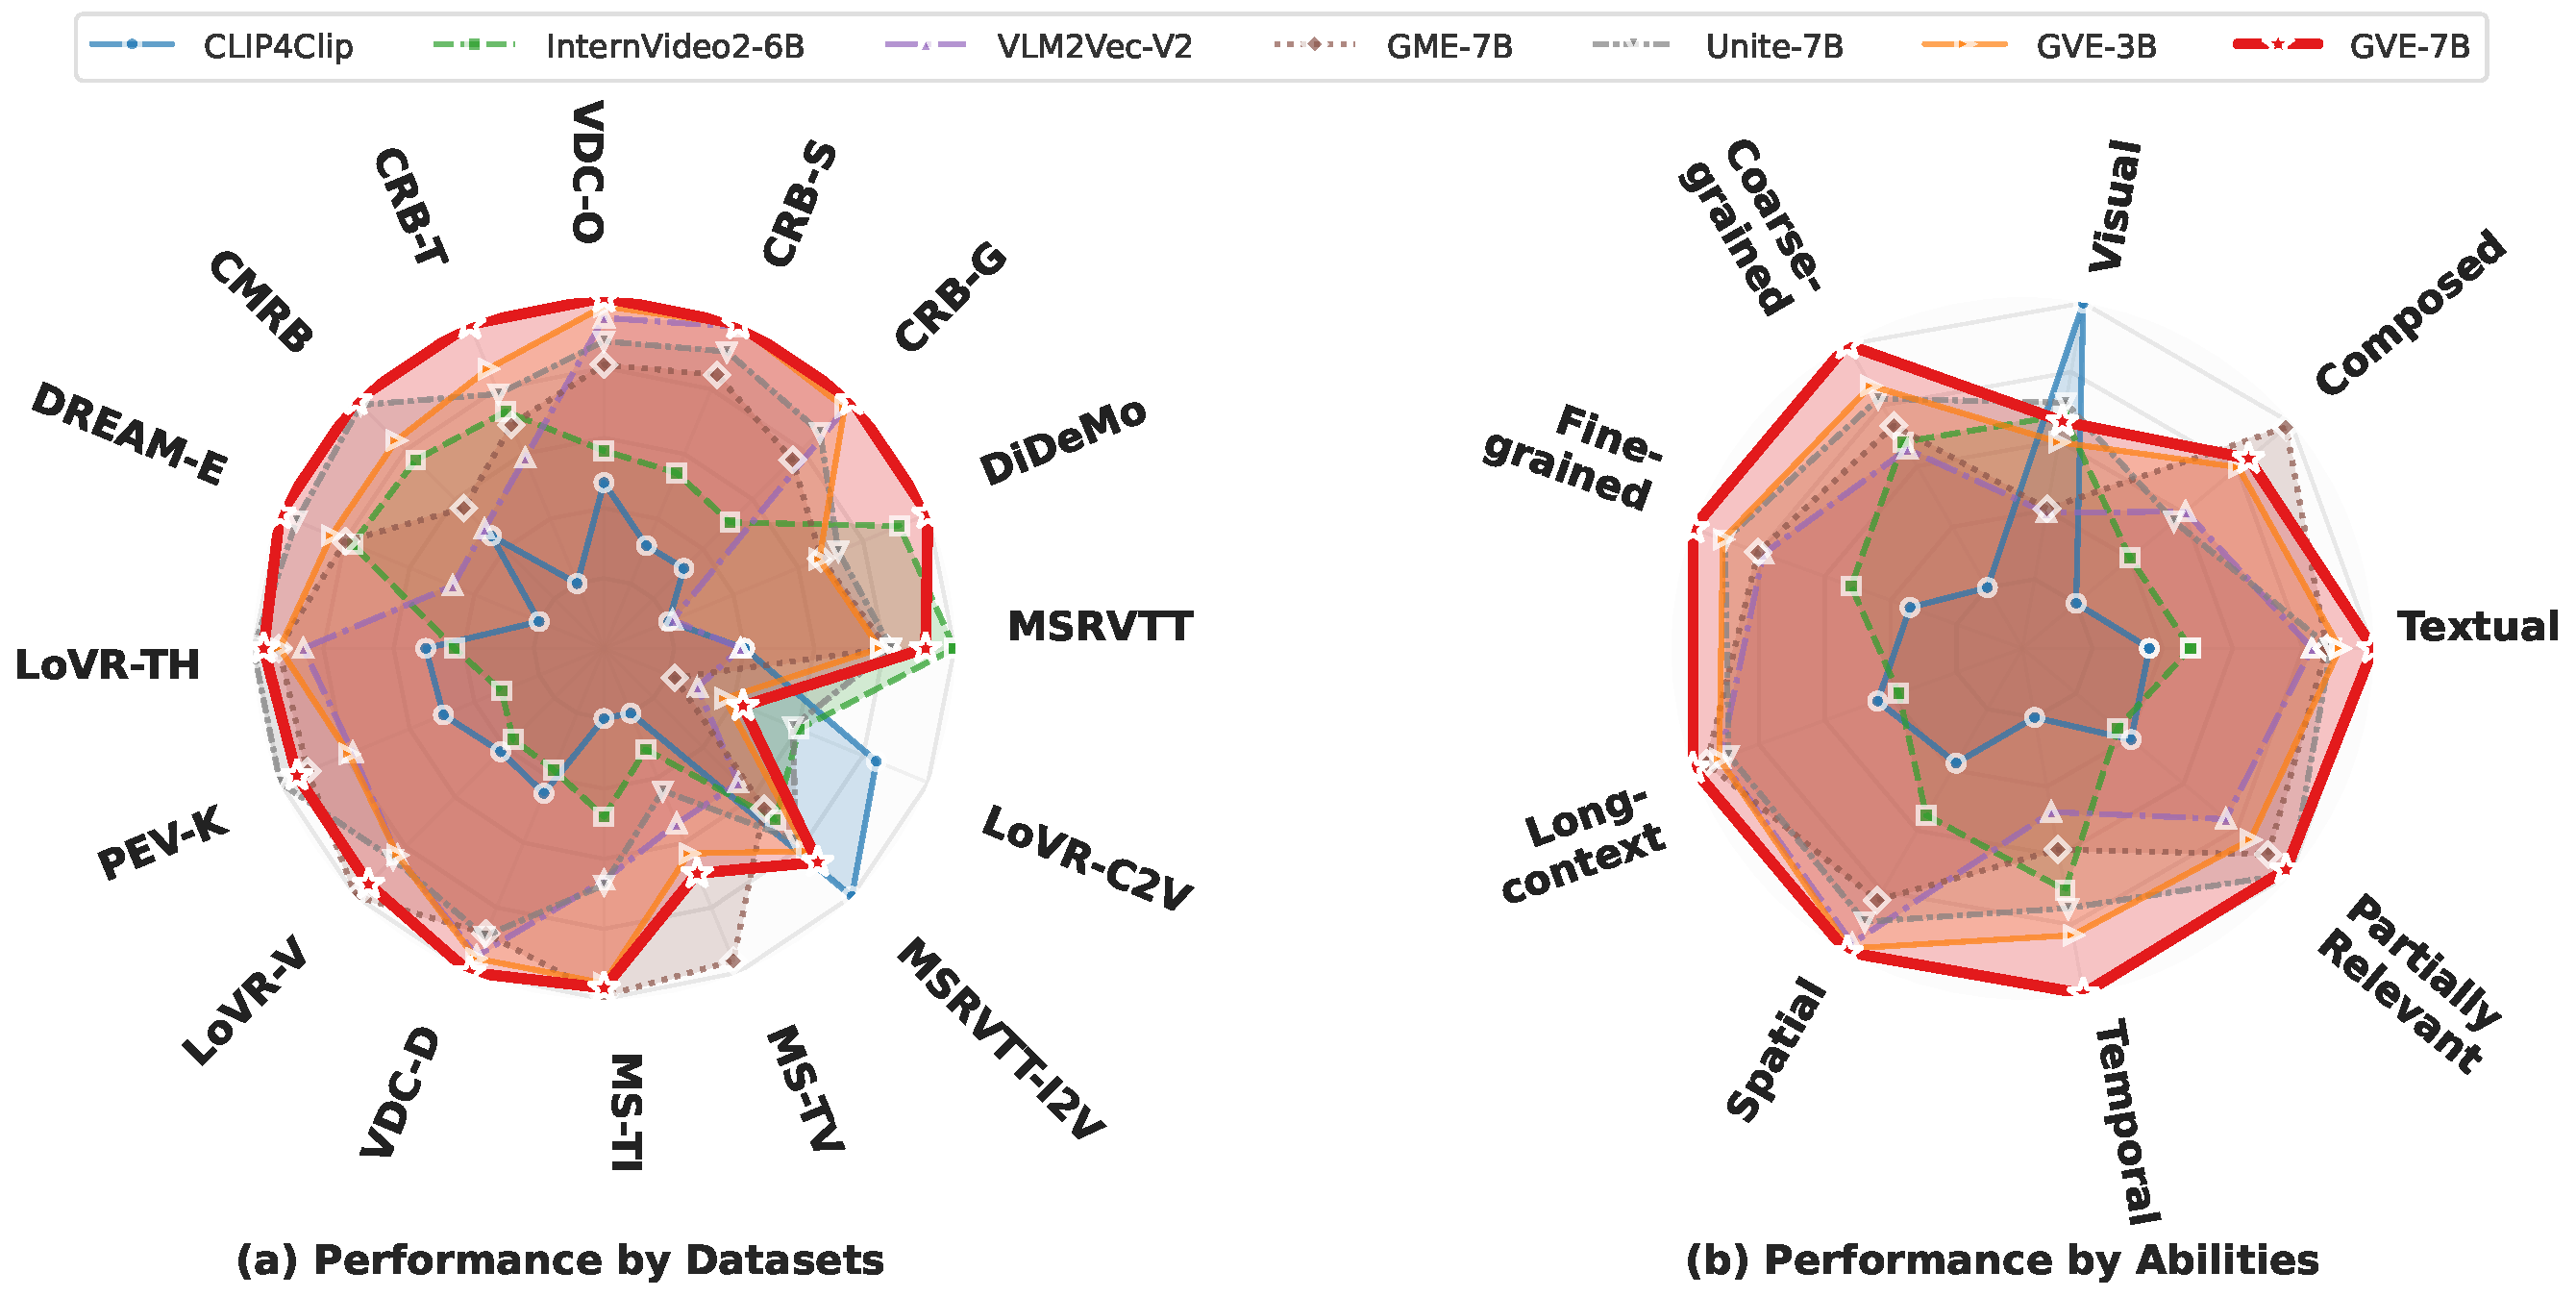
\includegraphics[width=\linewidth]{figures/gve/uvrb_dual_radar.pdf}
   \caption{Model performance on UVRB for 16 datasets and 9 abilities~(3 main tasks and 6 (sub-) domains).}
   \label{gve:fig:radar_uvrb}
\end{figure}

The contributions of this chapter are summarized as follows:
(1)~\textbf{Data}:~We propose V-SynFlow, a synthesis pipeline that produces UVRD with over $1.55$ million video-text pairs to explicitly address the data deficiencies identified in current models.
(2)~\textbf{Training}:~We introduce the Modality Pyramid curriculum, a training strategy that mitigates modality interference in heterogeneous multi-task learning, enabling the GVE model to achieve stable and strong zero-shot generalization.
(3)~\textbf{Analysis}:~Rather than proposing a novel benchmark, we establish a unified evaluation protocol across $16$ existing datasets. This standardized assessment systematically diagnoses model universality and offers new empirical insights beyond traditional evaluation paradigms.


\begin{figure}[t]
    \centering
    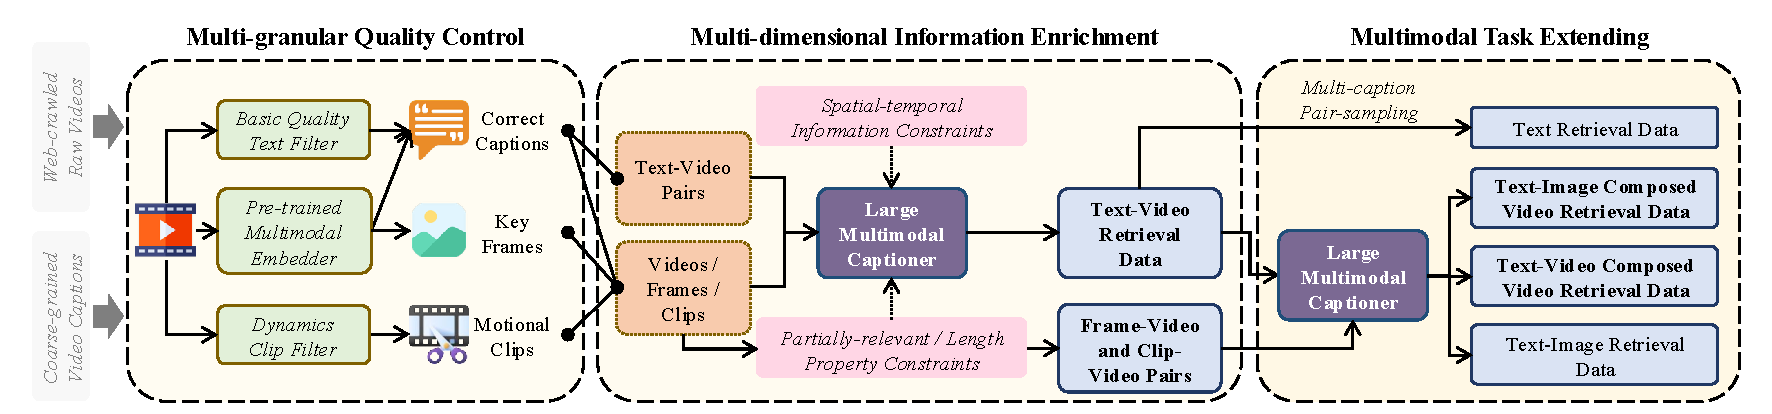
\includegraphics[width=\linewidth]{figures/gve/v-synflow.pdf}
    \caption{V-SynFlow: a multi-stage synthesis workflow for diverse video retrieval data.}
    \label{gve:fig:v-synflow}
\end{figure}

\section{Preliminary}\label{gve:sec:uvrb}

To bridge the persistent gap of fragmented evaluation protocols, we formulate the core problem from a holistic perspective by introducing the unified paradigm of Universal Video Retrieval~(UVR). This preliminary setup provides an objective diagnostic foundation to motivate our method contributions.

\subsection{Formulations}

The general ranking formulation in \S\ref{sec:bc-vr} is instantiated here across heterogeneous query formats and semantic domains. The query $q$, target video $v$, and cosine relevance score retain the meanings defined in Chapter~\ref{ch:related-work}. Here, the shared model $E_\theta$ instantiates the query and video embedding functions for heterogeneous inputs. UVR extends their scope by requiring consistent relevance ordering across the capability space defined below.

\begin{definition}[\textbf{Universal Video Retrieval~(UVR)}]\label{gve:def:universal_video_retrieval}
    Given a matching pair comprising a query $q$ and a video $v$, UVR aims to learn a $\theta$-parameterized model $E_\theta(\cdot)$ to compute a relevance score $s_{q \to v} = \cos(E_\theta(q), E_\theta(v))$. This score must be consistently higher than the similarity scores of irrelevant pairs across the query formats and data domains in the capability space defined below.
    Specifically, this paradigm categorizes the retrieval space into two primary dimensions:
    \textbf{(1)~Query Format} incorporates Textual~(TXT, e.g., natural language), Composed~(CMP, combinations such as text and image or text and video), and Visual~(VIS, pure image or video queries).
    \textbf{(2)~Data Domain} incorporates Coarse-grained~(CG, high-level semantics), Fine-grained categories including Spatial~(S, object), Temporal~(T, dynamics), and Partially Relevant~(PR, partial information), alongside Long-context~(LC, lengthy inputs).
\end{definition}

This formalization integrates isolated retrieval tasks into a comprehensive taxonomy, delineating the full spectrum of capabilities required for a truly universal video retrieval system.

\subsection{Unified Evaluation Protocol}

To operationalize the UVR paradigm and systematically diagnose generalization bottlenecks, we establish a standardized evaluation protocol across $16$ public video retrieval datasets. The consolidation of these existing resources into a unified evaluation suite, which we refer to as the Universal Video Retrieval Benchmark~(UVRB) protocol, provides a comprehensive framework for assessing model universality against the exhaustive query formats and domain complexities outlined in Definition~\ref{gve:def:universal_video_retrieval}.

To guarantee an objective assessment, all datasets undergo identical preprocessing, including uniform frame sampling, query normalization per task type, and strict adherence to a vision-only input scope. The evaluation follows a strictly model-agnostic protocol. Embeddings are extracted directly from the frozen representation space, and relevance is computed solely via cosine similarity without task-specific post-processing or learnable projections. This standardization eliminates heuristics and isolates the visual-semantic alignment capabilities of the backbones.

This comprehensive diagnostic framework exposes systemic capability deficiencies across current models, directly motivating the targeted data synthesis pipeline and heterogeneous task curriculum introduced in the subsequent methodology. The benchmark composition, dataset preparation, and execution pipeline are detailed below.

\subsubsection{Benchmark Composition and Dataset Preparation}

Figure~\ref{gve:fig:uvrb} visualizes how the 16 datasets cover the UVR capability space. Table~\ref{gve:tab:uvrb_dataset} summarizes their query and corpus sizes, video durations, and text lengths. All videos are evaluated using eight uniformly sampled frames. The datasets are grouped by query format and semantic domain according to Definition~\ref{gve:def:universal_video_retrieval}.

\begin{figure}[t]
    \centering
    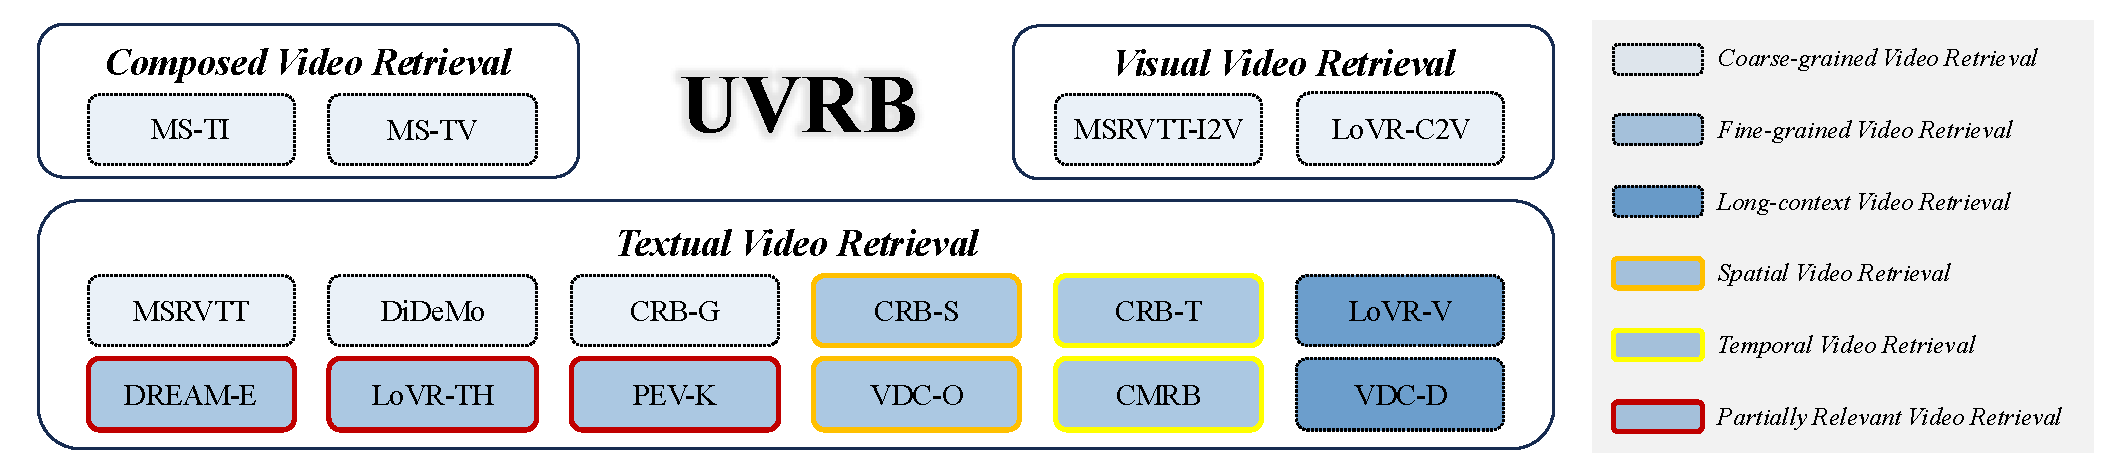
\includegraphics[width=\linewidth]{figures/gve/uvrb.pdf}
    \caption{Organization of the 16 public datasets in UVRB by query format and retrieval capability.}
    \label{gve:fig:uvrb}
\end{figure}

\begin{table}[t]
\centering
\caption{Statistics of the datasets in UVRB. All videos use eight uniformly sampled frames. Dur. denotes duration in seconds, and \# Word denotes query length in words.}
\label{gve:tab:uvrb_dataset}
\begin{tabular}{l r r r r}
\toprule
\textbf{Dataset} & \textbf{\# Query} & \textbf{\# Corpus} & \textbf{Dur.} & \textbf{\# Word} \\
\midrule
\multicolumn{5}{l}{\textbf{Textual Video Retrieval (Coarse-grained)}} \\
MSRVTT~\cite{xu2016msr} & 1,000 & 1,000 & 15.0 & 9.4 \\
DiDeMo~\cite{anne2017localizing} & 1,004 & 1,004 & 53.9 & 29.1 \\
CaReBench-General (CRB-G)~\cite{xu2025carebench} & 1,000 & 1,000 & 14.4 & 232.2 \\
\midrule
\multicolumn{5}{l}{\textbf{Textual Video Retrieval (Fine-grained Spatial)}} \\
CaReBench-Spatial (CRB-S)~\cite{xu2025carebench} & 1,000 & 1,000 & 14.4 & 115.0 \\
VDC-Object (VDC-O)~\cite{chai2024auroracap} & 1,027 & 1,027 & 30.1 & 91.4 \\
\multicolumn{5}{l}{\textbf{Textual Video Retrieval (Fine-grained Temporal)}} \\
CaReBench-Temporal (CRB-T)~\cite{xu2025carebench} & 1,000 & 1,000 & 14.4 & 103.2 \\
CameraBench (CMRB)~\cite{lin2025towards} & 728 & 1,071 & 5.7 & 24.8 \\
\multicolumn{5}{l}{\textbf{Textual Video Retrieval (Partially Relevant)}} \\
DREAM-1K-Event (DREAM-E)~\cite{wang2024tarsier} & 6,251 & 1,000 & 8.8 & 6.5 \\
LoVR-Theme2Clip (LoVR-TH)~\cite{cai2025lovr} & 8,854 & 8,854 & 16.9 & 48.1 \\
PE-Video-Keyword (PEV-K)~\cite{bolya2025perception} & 14,427 & 15,000 & 16.9 & 45.5 \\
\midrule
\multicolumn{5}{l}{\textbf{Textual Video Retrieval (Long-context)}} \\
LoVR-Text2Video (LoVR-V)~\cite{cai2025lovr} & 100 & 467 & 1560.3 & 17364.5 \\
VDC-Detail (VDC-D)~\cite{chai2024auroracap} & 1,000 & 1,027 & 30.1 & 508.0 \\
\midrule
\multicolumn{5}{l}{\textbf{Composed Video Retrieval}} \\
MomentSeeker-Text-Image (MS-TI)~\cite{yuan2025momentseeker} & 400 & 10 & 13.5 & 68.5 \\
MomentSeeker-Text-Video (MS-TV)~\cite{yuan2025momentseeker} & 400 & 10 & 13.5 & 68.5 \\
\midrule
\multicolumn{5}{l}{\textbf{Visual Video Retrieval}} \\
MSRVTT-ImageVideo (MSRVTT-I2V)~\cite{xu2016msr} & 1,000 & 1,000 & 15.0 & -- \\
LoVR-Clip-to-Video (LoVR-C2V)~\cite{cai2025lovr} & 467 & 467 & 1560.3 & -- \\
\bottomrule
\end{tabular}
\end{table}

We use the JSFusion split of MSRVTT~\cite{yu2018joint} and concatenate all descriptions of each DiDeMo video following~\cite{liu2019use}. For CaReBench, the general, spatial, and temporal caption fields define CRB-G, CRB-S, and CRB-T, respectively. VDC-O uses the object-centric captions from VDC, while CMRB uses camera-motion descriptions. DREAM-E, LoVR-TH, and PEV-K use event descriptions, theme annotations, and keyword fields to evaluate partially relevant retrieval. LoVR-V and VDC-D use long-form and detailed captions for long-context retrieval. Following the MomentSeeker adaptation in~\cite{meng2025vlm2vec}, MS-TI and MS-TV combine text with an image or a video clip to retrieve a target clip. For visual retrieval, MSRVTT-I2V uses one randomly sampled frame as the query, and LoVR-C2V uses a short clip to retrieve its source long video.

Table~\ref{gve:tab:uvrb_prompts_metric} lists the instruction and metric for each dataset. This explicit mapping keeps instruction-sensitive models under a common task definition while preserving the metric appropriate to each benchmark.

\begin{table}[t]
\centering
\caption{Query instructions and metrics for the datasets in UVRB.}
\label{gve:tab:uvrb_prompts_metric}
\begin{tabular}{l p{10cm} l}
\toprule
\textbf{Dataset} & \textbf{Query Instruction} & \textbf{Metric} \\
\midrule
MSRVTT & Find the clip that corresponds to the described scene in the given video. & R@1 \\
DiDeMo & Find a video that includes the following described scenes. & R@1 \\
CRB-G & Find the video according to the general text description. & R@1 \\
CRB-S & Find the video according to the spatial description. & R@1 \\
VDC-O & Find the video according to the object description. & R@1 \\
CRB-T & Find the video according to the temporal description. & R@1 \\
CMRB & Find the video according to the camera motion description. & R@10 \\
DREAM-E & Find the video according to the text description. & R@1 \\
LoVR-TH & Find the video according to text description about video theme information. & R@10 \\
PEV-K & Find the video according to the text description of a series of keywords. & R@1 \\
LoVR-V & Find the long video according to the long text description. & R@1 \\
VDC-D & Find the video according to the detailed text description. & R@1 \\
MS-TI & Find the video clip that corresponds to the given text and image. & P@1 \\
MS-TV & Find the video clip that corresponds to the given text and video. & P@1 \\
MSRVTT-I2V & Find the video according to the image. & R@1 \\
LoVR-C2V & Find the original long video according to the short video clip. & R@1 \\
\bottomrule
\end{tabular}
\end{table}

\subsubsection{Evaluation Pipeline}

The evaluation is implemented on MTEB~\cite{muennighoff2022mteb} and decouples the evaluation engine from the model architecture through a standardized interface. It proceeds through dynamic task orchestration, configurable model execution, and metric and diagnostic generation. Domain-specific prompts are injected for instruction-sensitive tasks, while dedicated loaders integrate custom benchmarks. Expensive tasks can be deferred, and model initialization abstracts precision and multi-GPU configuration. The data layer supports online and offline modes, and explicit multi-GPU management and clean shutdown handling improve reliability for large-scale evaluation.


\section{Methodology}

This section introduces a co-designed framework for universal video retrieval. Guided by UVR, we first propose V-SynFlow. This workflow synthesizes the Universal Video Retrieval Dataset~(UVRD), comprising $1.55$ million targeted video-text pairs to explicitly supplement general retrieval data. Subsequently, we introduce the \pyramid curriculum, a strategy designed to stabilize the optimization of the General Video Embedder~(GVE) by leveraging inherent task hierarchies across heterogeneous modalities.

\subsection{Scalable Synthesis of Cross-Domain Multi-Task Video Retrieval Data}\label{gve:sec:data_synthesis}
Training a universal video embedder is fundamentally impeded by a deficiency of high-quality supervision for divergent tasks. Guided by the concrete capability gaps identified in the preliminary diagnostics, such as severe shortcomings in fine-grained temporal reasoning and composed retrieval, we introduce \textbf{V-SynFlow}~(Figure~\ref{gve:fig:v-synflow}). This pipeline transforms weakly annotated web videos from raw datasets~(e.g., PVD~\cite{bolya2025perception}, InternVid-FLT~\cite{wang2023internvid}, and WebVid~\cite{bain2021frozen}) into structured, high-fidelity, and gap-targeted multi-task training instances. Through this targeted approach, we construct the \textbf{Universal Video Retrieval Dataset~(UVRD)}, containing over $1.55$ million descriptive pairs tailored for multidimensional training enhancement.
Specifically, the V-SynFlow workflow proceeds in three stages as follows. The construction implementation and complete generation prompts are provided after the three stages.

\paragraph{Multi-granular Quality Control.}
Given a raw corpus $\mathcal{D} = \{(v_i, t_i)\}$, we produce a high-fidelity asset pool, $\mathcal{A}_{tfc}$. The process applies a filter cascade. \textit{Annotation Rectification} removes non-descriptive text. \textit{Cross-Modal Consistency Filtering} discards pairs where the similarity measured by a pretrained embedder $\Phi(\cdot)$~(e.g., GME-7B~\cite{Zhang_2025_CVPR}) falls below a predefined threshold, empirically set to 0.25. \textit{Temporal Dynamics Filtering} removes static content to ensure sufficient temporal signals. The resulting asset pool $\mathcal{A}_{tfc}$ contains a set of validated videos $\{v_j\}$, the original captions $\{t_j\}$, and corresponding sets of extracted frames $\{f_{jk}\}$ alongside cropped clips $\{c_{jl}\}$.

\begin{figure}[t]
    \centering
    \begin{minipage}[b]{0.7\textwidth}
        \centering
        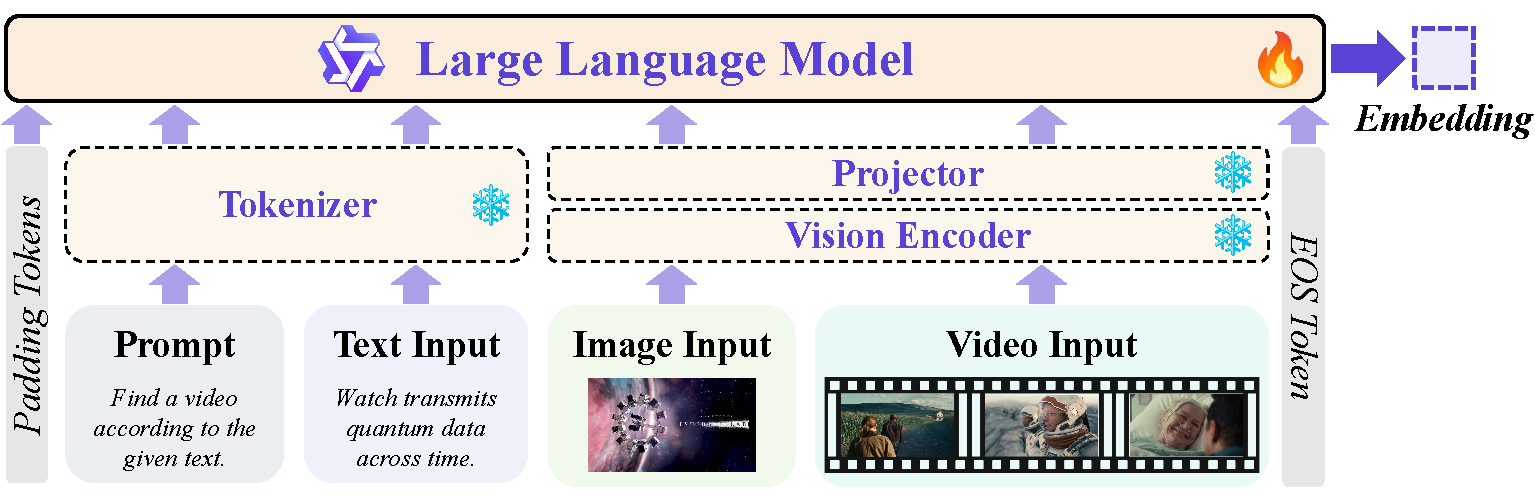
\includegraphics[width=\linewidth]{figures/gve/model.pdf}
        \caption{The architecture of GVE, an MLLM-based embedding model. We fine-tune only the LLM component. GVE accepts compositional multimodal inputs and produces a high-dimensional embedding.}
        \label{gve:fig:model}
    \end{minipage}
    \hfill
    \begin{minipage}[b]{0.26\textwidth}
        \centering
        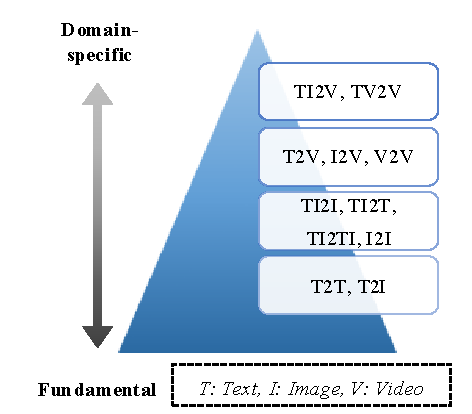
\includegraphics[width=\linewidth]{figures/gve/modality-pyramid.pdf}
        \caption{\pyramid: simpler tasks lay the foundation for specific ones.}
        \label{gve:fig:pyramid}
    \end{minipage}
\end{figure}

\paragraph{Multi-dimensional Information Enrichment.}
We leverage the filtered assets within $\mathcal{A}_{tfc}$ to generate richer data structures. To create an enriched text-video dataset $\mathcal{D}^{+}$, we utilize an MLLM, $\mathcal{M}_{\text{cap}}$~(e.g., Keye-VL-8B~\cite{team2025kwai}), as a conditional captioning engine. For each video $v_j$, the engine synthesizes multiple captions $\{t^{'}_{jk}\}$ conditioned by diagnostic-driven information profiles. Specifically, because the diagnostic evaluation revealed a pronounced spatial-temporal decoupling wherein temporal skills constitute the primary bottleneck, we deliberately skew the synthesis distribution: $60\%$ temporal, $30\%$ spatial, and $10\%$ targeted at partially relevant or abstract semantics, informed by our preliminary diagnostic results on UVRB. By sampling one caption for each video, we obtain a set of novel high-quality text-video pairs $\{(v_j, t^{'}_{jk})\}$. Furthermore, we pair videos with the corresponding visual components to construct collections of visual pairs $\mathcal{P}_{f \leftrightarrow v}$ and $\mathcal{P}_{c \leftrightarrow v}$, resulting in frame-to-video $\{(f_{jk}, v_j)\}$ and clip-to-video $\{(c_{jl}, v_j)\}$ instances. To mitigate potential hallucination biases inherent in generative MLLMs, we enforce strict instructional prompts and rely on the aforementioned cross-modal consistency filtering to automatically discard misaligned generations.

\paragraph{Multimodal Task Extension.}
The final stage assembles the unified training corpus, $\mathcal{D}_{\star}$. To explicitly address the composed retrieval deficiency, we synthesize complex composed tasks by leveraging $\mathcal{P}_{f \leftrightarrow v}$ and $\mathcal{P}_{c \leftrightarrow v}$. For each visual pair, such as $(f_{jk}, v_j)$, the engine $\mathcal{M}_{\text{cap}}$ generates a query text $t^{f_{jk} \to v_j}$ describing the temporal evolution, forming a training instance $((t^{f_{jk} \to v_j}, f_{jk}), v_j)$. Additionally, basic alignment tasks (e.g., text-image pairs) are sampled from $\mathcal{A}_{tfc}$. For each video, two candidates from the unselected synthesized captions are mapped as text-to-text pairs. The resulting dataset $\mathcal{D}_{\star}$ provides the comprehensive mixture of tasks essential for training a universal embedder.

\paragraph{Dataset-Construction Implementation.}
To support scalable and reproducible construction across these task types, we implement V-SynFlow as a unified object-oriented framework. Every retrieval task is represented by a canonical tripartite abstraction comprising a \textsc{Corpus}, a set of \textsc{Queries}, and a \textsc{Relevance Mapping}. An abstract base class enforces this structural invariant across text-to-video, visual, and composed retrieval datasets.

The framework supports three forms of specialization. First, modality is treated as configuration, allowing a dataset to transition among text, image, video, and composite queries by overriding its modality-specific access method. Second, complex tasks are derived through inheritance. For example, a text-and-image-to-video task extends a base retrieval task with an additional query component, while dataset variants override only the required data-access methods. Third, large sources such as InternVid-FLT are processed in parallel chunks, with automated validators checking resolution, frame count, and video integrity. Common media errors are repaired using \texttt{ffmpeg}, reducing the risk that downstream failures originate from corrupted input rather than retrieval difficulty.

\subsubsection{Prompt Specifications for Synthetic Data Generation}\label{gve:sec:prompt_specs}

To ensure high-quality, diverse, and controllable synthetic video retrieval data generation at scale, we design and deploy a suite of structured prompts to instruct MLLMs for captioning. Our pipeline operates in four parts:

\begin{enumerate}
    \item \textbf{Raw~(Or Weakly Annotated) Video (Re-)~Captioning}: Enhance raw or uncaptioned videos with rich, diverse textual descriptions.
    \item \textbf{Text-Image Composed Retrieval}: Generate queries that combine reference images with video content for fine-grained retrieval.
    \item \textbf{Text-Video Composed Retrieval}: Generate queries that combine short reference clips with target videos for practical temporal or perspective-based retrieval.
    \item \textbf{Frame Image Captioning}: Annotate individual video frames with dynamic-aware captions for auxiliary training signals.
\end{enumerate}

All prompts enforce strict output formatting, factual grounding, and stylistic diversity to ensure dataset quality and coverage. \texttt{\{raw\_caption\}} represents an optional, potentially low-quality human-provided or auto-generated caption associated with the video. Placeholders (e.g., \texttt{\{readability\}} and \texttt{\{education\_level\}}) are dynamically instantiated during batch generation.

We also generate text-to-text retrieval data by randomly pairing two descriptions from the video or frame caption list.

% ========================================
% Prompt 1: Video Captioning
% ========================================
\begin{promptbox}{Synthetic Video Captioning Prompt}
\begin{lstlisting}[style=promptstyle]
Generate 5 distinct and high-quality ENGLISH captions for the provided video. Please first visually understand the video file and analyze the video frame-by-frame in depth before captioning.

The original video caption is {raw_caption}. (Ignore if empty.)

Each caption must be:
  1. The final answer MUST only be a JSON dict of captions where the key is the caption number and the value is a single-paragraph caption.
  2. Factually accurate and descriptive - include only what is clearly visible or reasonably inferable from the video.
  3. Focus exclusively on visible content; do not mention absences or speculate about unseen elements.

Content Requirements (per caption):
  1. Spatial Details (30-60%): Describe location, setting, key environmental elements, objects, and their spatial relationships. Include notable visual features.
  2. Temporal Flow (30-60%): Capture event sequence and action dynamics - movements, interactions, transitions - as they unfold over time.
  3. Theme/Background/Style/Meaning/Highlight/Camera (0-20%): Describe observable emotional tone, narrative style, thematic elements, highlighting frames, or significant camera movements/angles.
  4. Others (0-10%).

Key Guidelines:
  1. Do not invent fictional elements, dialogue, or backstory not visible in the video.
  2. Use the following varied sentence styles (one per caption):
       - concise and punchy summary,
       - spatial-temporal richly descriptive,
       - abstract understanding,
       - keywords-only,
       - partially relevant information.
  3. Ensure diversity: avoid repetition in wording, focus, or rhythm; at least one caption must be <20 words and one >100 words; balance objectivity with vivid sensory language; randomly omit minor details in 1 or 2 captions.
  4. Ensure readability matches {readability} and is appropriate for {education_level} readers.

Now generate these captions in strict JSON format:
{
   "1": <caption text 1: concise and punchy summary, 10-25 words>,
   "2": <caption text 2: spatial-temporal richly descriptive, 80-200 words>,
   "3": <caption text 3: abstract understanding, 30-100 words>,
   "4": <caption text 4: keywords-only, 5-30 words>,
   "5": <caption text 5: partially relevant information, 10-70 words>
}
\end{lstlisting}
\end{promptbox}

% ========================================
% Prompt 2: Text-Image Composed Retrieval
% ========================================
\begin{promptbox}{Synthetic Text-Image Composed Video Retrieval Prompt}
\begin{lstlisting}[style=promptstyle]
You are an information retrieval expert specializing in high-value text-image composed queries. Your sole objective is to generate queries that significantly enhance video retrieval performance by effectively combining a reference image and video content.

## What Makes a HIGH-QUALITY Query (Non-Negotiable)
A truly valuable query must satisfy ALL of these criteria:

1. COMBINATION NECESSITY (Most Critical)
   - The query MUST become meaningless or significantly less specific if either the image or video is removed.
   - Example (HIGH-QUALITY): "the person FROM REFERENCE IMAGE wearing red jacket now skiing"
   - Example (LOW-QUALITY): "a person skiing" (works without image)

2. SEMANTIC PRECISION
   - Must accurately reflect BOTH the visual content of the reference image AND the video.
   - Must reference at least ONE specific visual attribute from the image (not generic descriptions).
   - Example (HIGH-QUALITY): "matching the blue hat FROM PHOTO, now running through park"
   - Example (LOW-QUALITY): "someone similar to image moving" (too vague)

3. RETRIEVAL EFFECTIVENESS
   - Must narrow search results by at least 50\% compared to text-only queries.
   - Must contain actionable constraints that differentiate from 90\% of videos in the database.
   - Example (HIGH-QUALITY): "the woman WITH PONYTAIL FROM IMAGE entering building at 2PM"
   - Example (LOW-QUALITY): "a woman walking" (too broad)

4. LOGICAL COHERENCE
   - Must maintain subject-verb-object consistency across modalities.
   - Must avoid semantic contradictions between image attributes and video actions.
   - Example (HIGH-QUALITY): "the dog FROM REFERENCE PHOTO chasing a ball"
   - Example (LOW-QUALITY): "the red jacket FROM IMAGE running down hill" (jackets don't run)

5. PRACTICAL UTILITY
   - Must solve a real-world ambiguity that neither text nor image could resolve alone.
   - Must reflect how actual users would express their information need.
   - Example (HIGH-QUALITY): "same person AS IN PHOTO but wearing blue instead of red"
   - Example (LOW-QUALITY): "the image shows a person and the video shows action" (no real combination)

## High-Value Query Generation Framework
Follow this structured approach:

1. DEEP ANALYSIS PHASE (Mandatory)
   a) Reference Image Analysis:
      - Identify 1-4 SPECIFIC visual attributes (e.g., "red jacket", "ponytail", "blue hat")
      - Determine primary subject with discriminative features
      - Note what CANNOT be determined from image (e.g., action, scene)

   b) Video Content Analysis:
      - Identify primary action using precise verbs (e.g., "running", "entering", "chasing")
      - Note scene context and temporal elements
      - Determine what CHANGES from the static image reference

2. COMBINATION STRATEGY SELECTION
   Choose ONE primary strategy:

   A) IDENTITY PRESERVATION + ACTION CHANGE
      - Structure: [Binding phrase] + [Image attribute] + [Video action]
      - Example: "the man FROM REFERENCE IMAGE in blue shirt now running"

   B) IDENTITY PRESERVATION + SCENE MIGRATION
      - Structure: [Binding phrase] + [Image attribute] + [Scene transition]
      - Example: "same person AS IN PHOTO moving from office to park"

   C) IDENTITY PRESERVATION + NEGATIVE CONSTRAINT
      - Structure: [Binding phrase] + [Negative constraint] + [Video state]
      - Example: "not wearing red jacket FROM IMAGE but blue, walking"

   D) RELATIONAL TRANSFER
      - Structure: [Binding phrase] + [Relationship description]
      - Example: "the dog FROM REFERENCE PHOTO chasing a ball"

3. QUALITY ENHANCEMENT TECHNIQUES
   - Binding Precision: Use "FROM REFERENCE IMAGE", not "like the picture"
   - Attribute Specificity: Use concrete features ("red jacket", not "clothing")
   - Action Verbs: Use present continuous tense ("running", not "runs")
   - Context Enrichment: Add 1 relevant scene descriptor ("in park", "near building")
   - Noise Handling: For low-quality inputs, use "resembling" but maintain specificity
   - Audience Adaptation: Ensure readability matches {readability} and suits {education_level} readers.

4. MANDATORY QUALITY CHECK
   Before finalizing, verify ALL:
   - [ ] Explicit binding to reference image
   - [ ] References SPECIFIC visual attribute from image
   - [ ] Describes DYNAMIC ELEMENT not in static image
   - [ ] Loses specificity if image removed
   - [ ] Contains actionable retrieval constraint
   - [ ] Maintains logical subject-action consistency
   - [ ] Solves real-world ambiguity

## What to AVOID
- Generic descriptions ignoring image specificity
- Redundant mentions of obvious image content
- Semantic contradictions (e.g., "the jacket is running")
- Overly precise details not visible in inputs
- Standalone video descriptions without image binding
- Vague terms: "something", "thing", "area"
- Excessive length without added value (>50 words)

## Output Format
- Output ONLY a JSON object with one key: "query"
- Value must be the generated query sentence
- No additional text or formatting

Generate the query for:
Reference Image: <image_input>
Video Clip: <video_input>
\end{lstlisting}
\end{promptbox}

% ========================================
% Prompt 3: Text-Video Composed Retrieval
% ========================================
\begin{promptbox}{Synthetic Text-Video Composed Video Retrieval Prompt}
\begin{lstlisting}[style=promptstyle]
You are an information retrieval expert specializing in practical text-video composed queries. Your objective is to generate queries that effectively combine a short reference clip with a target video for real-world retrieval.

## Practical Context Understanding
In real-world scenarios:
- Reference is typically a SHORT CLIP (2-10 seconds)
- Clip is usually HIGHLY RELEVANT to target video (same source or similar content)
- Common relationships: temporal continuation, perspective variation, quality differences, minor action variations
- Query should reflect how users actually search

## What Makes a HIGH-QUALITY Query (Practical Focus)
Must satisfy these criteria:

1. USEFUL COMBINATION (Most Important)
   - Leverages reference clip to specify what text alone cannot
   - Example (HIGH-QUALITY): "the same person FROM REFERENCE CLIP continuing to run after the jump"
   - Example (LOW-QUALITY): "a person running" (ignores reference)

2. PRACTICAL PRECISION
   - References at least ONE observable feature from reference clip
   - Example (HIGH-QUALITY): "matching the red jacket FROM REFERENCE, now entering building"
   - Example (LOW-QUALITY): "someone similar to clip moving" (too vague)

3. REAL-WORLD UTILITY
   - Helps find videos difficult to retrieve with text alone
   - Example (HIGH-QUALITY): "same action AS IN REFERENCE but from front angle"
   - Example (LOW-QUALITY): "the clip shows action" (no retrieval value)

4. NATURAL EXPRESSION
   - Sounds like how a real user would phrase it
   - Example (HIGH-QUALITY): "what happens right after this moment?"
   - Example (LOW-QUALITY): "temporal continuation of the current visual sequence" (too academic)

## Practical Query Generation Framework

1. REFERENCE CLIP ANALYSIS
   - Identify 1-3 KEY OBSERVABLE FEATURES (e.g., "red jacket", "starting pose", "mid-action")
   - Determine most distinctive visual or action element
   - Note what is CLEARLY VISIBLE (avoid guessing)

2. TARGET VIDEO RELATIONSHIP ASSESSMENT
   Determine relationship type:

   A) TEMPORAL CONTINUATION
      - Reference is earlier part of same sequence
      - Query focus: "what happens next" or "continuing action"

   B) PERSPECTIVE VARIATION
      - Same action from different angle/view
      - Query focus: "same action from different angle"

   C) QUALITY/CONDITION VARIATION
      - Same action with different lighting/resolution
      - Query focus: "same scene in better lighting"

   D) MINOR ACTION VARIATION
      - Slightly different execution of similar action
      - Query focus: "same person but running instead of walking"

3. QUERY CONSTRUCTION
   - Start with binding phrase: "FROM REFERENCE CLIP", "AS IN REFERENCE", etc.
   - Reference 1-2 specific observable features from clip
   - Describe relationship to target video clearly
   - Keep natural and practical (5-15 words typically)
   - For temporal: focus on "what happens next"
   - For perspective: specify desired viewpoint
   - For quality: specify desired condition
   - For action: specify the change

4. PRACTICAL QUALITY CHECK
   Ask before finalizing:
   - Would this help me find what I'm looking for?
   - Does it add value beyond describing the target?
   - Would a real user phrase it this way?
   - Is everything mentioned clearly visible in reference?

## What to AVOID
- Overly academic or technical language
- References to features NOT clearly visible
- Excessive precision about timing ("exactly 3.2 seconds later")
- Queries that work equally well without reference
- Generic descriptions: "similar video", "related content"
- Making unsupported assumptions

## Output Format
- Output ONLY a JSON object with key: "query"
- Value must be the generated query string
- No additional text, explanations, or formatting

Generate the query for:
Reference Clip: <reference_clip_input>
Target Video: <target_video_input>
\end{lstlisting}
\end{promptbox}

% ========================================
% Prompt 4: Frame Captioning
% ========================================
\begin{promptbox}{Synthetic Frame Captioning Prompt}
\begin{lstlisting}[style=promptstyle]
Generate 5 distinct and high-quality ENGLISH captions for the provided image (a frame extracted from a video) based solely on visual content. Please first visually understand the image and analyze it in depth before captioning.

Each caption must be:
  1. The final answer MUST only be a JSON dict of captions where the key is the caption number and the value is a single-paragraph caption.
  2. Factually accurate and descriptive - include only what is clearly visible; captions should also be consistent with the short-term video context.
  3. Focus exclusively on visible content; do not mention absences or speculate about unseen context.

Content Requirements (per caption):
  1. Spatial Details (50-70%): Describe location, setting, key objects, spatial relationships, colors, lighting, composition. Include instantaneous action states derived from visible posture/motion cues.
  2. Temporal Snapshots (0-30%): Describe the frozen moment's temporal state (movements, interactions, transitions) ONLY if visually provable. Avoid implying sequence, duration, or speed.
  3. Theme/Style/Composition (10-20%): Cover emotional tone, camera angle, lighting style, or artistic elements directly observable.
  4. Others (0-10%).

Key Guidelines:
  1. Do not invent fictional elements or backstory. If action is ambiguous, describe neutrally. Never use future/past tense or speculative phrases.
  2. Use varied sentence styles (randomly assign one per caption):
       - concise spatial-temporal snapshot,
       - spatially rich descriptive,
       - abstract spatial interpretation,
       - keywords with temporal anchors,
       - minimalist spatial focus.
  3. Ensure diversity: avoid repetition in wording, focus, or rhythm; at least one caption <20 words and one >100 words; balance objectivity with vivid sensory language; randomly omit minor details in 1-2 captions.
  4. Ensure readability matches {readability} and is appropriate for {education_level} readers.

Now generate these captions in strict JSON format:
{
   "1": <caption text 1: concise and punchy summary, 10-25 words>,
   "2": <caption text 2: spatial-temporal richly descriptive, 50-200 words>,
   "3": <caption text 3: abstract understanding, 30-100 words>,
   "4": <caption text 4: keywords-only, 5-30 words>,
   "5": <caption text 5: partially relevant information, 10-70 words>
}
\end{lstlisting}
\end{promptbox}

\paragraph{Prompt Utilization.}
These prompts are designed for a scalable, schema-constrained generation pipeline for synthesizing diverse video-centric annotations and queries. The system unifies four tasks under a single modular framework.
Each task is governed by a structured prompt template with dynamic control slots (e.g., readability, education level), ensuring linguistic and semantic diversity. Input modalities (image, video, or both) are automatically routed and embedded via a distributed multimodal LLM (Keye-VL-8B~\cite{team2025kwai}, 32K context), with outputs rigorously validated against JSON schemas for structural correctness.
The pipeline supports sharded, resumable batch generation with quality-aware sampling, enabling the production of millions of grounded, stylistically varied synthetic instances.

\subsubsection{Human Validation}
To assess the quality of the automatically generated UVRD, human expert evaluation was conducted on a random sample of $100$ instances. Validation confirmed a 95\% factual accuracy rate. The five erroneous instances comprised two minor overclaims or underclaims of visual details, two minor inaccuracies in camera-motion descriptions, and one subtle temporal-ordering error. While this human-verified sample is a preliminary subset, it corroborates the efficacy of our automated multi-granular quality control pipeline, which serves as the primary scalable safeguard for the entire 1.55 million-pair corpus.


\subsection{Modality Pyramid: Customized Curriculum Contrastive Learning}
\label{gve:sec:modality_pyramid}

The synthesized dataset provides a rich mixture of retrieval tasks spanning diverse query formats and data domains. To embed these multimodal inputs into a unified space, we introduce the \textbf{General Video Embedder~(GVE)}~(Figure~\ref{gve:fig:model}), a multimodal encoder derived from Qwen2.5-VL~\cite{bai2025qwen25vl} to inherit the pretrained vision-language alignment of the backbone model.

\paragraph{GVE Architecture.}
For arbitrary modality combinations, GVE fuses tokenized prompt and text inputs with projected visual features into a joint sequence. Text is represented as $\mathbf{X}_t \in \mathbb{Z}^{B \times T_t}$, while images and video frames are encoded as $\mathbf{X}_v \in \mathbb{R}^{B \times T_v \times d}$. For images, $T_v=\mathrm{THW}/p_s^2$. For videos with $K$ uniformly sampled frames, $T_v=K\cdot(\mathrm{THW}/p_s^2)$, and absolute temporal encodings are added to the frame embeddings. The frame count satisfies $K \bmod p_t=0$, with $p_t=p_s=2$ by default, to maintain alignment with the 3D spatiotemporal grid of the vision encoder. Replacing the visual placeholders in the text sequence with these visual tokens produces $\mathbf{X}_{\mathrm{fused}} \in \mathbb{R}^{B \times T \times d}$, where $T=T_t+\sum T_v$. This scatter-based fusion preserves positional coherence for interleaved modality composition.

The LLM processes the fused sequence, and the embedding for the $i$-th instance is extracted from the last attended token and normalized as
\begin{equation}
    \mathbf{e}^{(i)} = \frac{\mathbf{h}^{(i)}_{p_i}}{\|\mathbf{h}^{(i)}_{p_i}\|_2}, \qquad
    p_i = \max \{j \mid \mathbf{M}^{(i)}_j=1\},
\end{equation}
where $\mathbf{M}^{(i)}$ is the attention mask. This position corresponds to the EOS token in left-padded sequences or the final non-padding token in right-padded sequences. The resulting fixed-dimensional representation supports retrieval across arbitrary modality compositions.

However, naively mixing this highly heterogeneous data leads to severe modality interference and optimization instability. In early training stages under random scheduling, gradient signals from complex temporal and composed tasks are frequently submerged by simpler spatial alignment tasks, leading to erratic loss convergence and suboptimal performance on complex tasks.
To ensure stable optimization across heterogeneous formats, we propose \textbf{Modality Pyramid}~(Figure~\ref{gve:fig:pyramid}), a curriculum that schedules training from atomic to composite tasks for progressive knowledge acquisition. This bottom-up design is grounded in empirical evidence: after a single epoch, a clear task hierarchy emerges based on alignment scores, descending from text-image ($0.65$) down to text-video ($0.46$) and composed video ($0.43$) tasks (Table~\ref{gve:tab:task_alignment}). The curriculum functions as a stabilizing strategy, guiding the embedding model to master perceptual primitives prior to advancing to complex integration, thereby mitigating gradient submergence.

\paragraph{Alignment-aware Dynamic Scheduling.}
At the beginning of each epoch $t$, we estimate the alignment of every task $k \in \mathcal{K}$ using a \textit{prober model} $\Psi_t$. For $t=1$, $\Psi_1$ is a robust off-the-shelf embedder (e.g., GME-7B~\cite{Zhang_2025_CVPR}). The selection of a robust, MLLM-based prober is deliberate to ground the curriculum in reliable and semantically rich task difficulty estimates for a stable initial anchor. For $t>1$, $\Psi_t$ utilizes the GVE checkpoint from the conclusion of epoch $t-1$. To prevent computational bottlenecks, this probing evaluation is performed offline using a randomly downsampled subset. For each task, we sample $N_p=1000$ positive pairs and compute the relevance score as the average cosine similarity:
\begin{equation*}
R_k^{(t)} = \frac{1}{N_p} \sum_i \cos\!\left(\Psi_t(x_i), \Psi_t(y_i)\right).
\end{equation*}
A higher $R_k^{(t)}$ indicates better current alignment.
During epoch $t$, tasks are sampled according to
\begin{equation*}
P^{(t)}(k) \propto \exp\!\left(\frac{R_k^{(t)}}{\sigma(t)}\right),
\end{equation*}
where the temperature $\sigma(t)$ increases linearly from $\sigma_{\min}$ to $\sigma_{\max}$ ($\sigma_{\min}=0.1$ and $\sigma_{\max}=1.0$ by default) across the total duration of the training epochs. This topological progression ensures an initial focus on well-aligned tasks while progressively encouraging challenging exploration.

\paragraph{Unified Contrastive Optimization.}
The GVE model is trained using a symmetric InfoNCE loss~\cite{oord2018representation} across all scheduled tasks. To strengthen discrimination, we augment in-batch negatives with hard negatives mined from a large external corpus utilizing the identical prober $\Psi_t$. To mitigate the risk of false negatives (i.e., visually similar but distinct videos that happen to share target semantics), we apply a strict similarity margin constraint during mining, discarding any candidates that exceed a similarity threshold of $0.90$ with the query. For a query–target pair $(q, v^+)$, the loss contrasts $v^+$ against both other positive samples in the batch and the top-$K$ retrieved hard negatives.
The similarity is computed as $s_{q \to v} = \cos(E_\theta(q), E_\theta(v))$, and the final loss is symmetrized over the query and target directions:
\begin{equation}
\mathcal{L}_{i}^{(q \to y)} = -\log
\frac{\exp(s_{q_i \to y_i^+}/\tau_l)}
{\exp(s_{q_i \to y_i^+}/\tau_l) + \sum_{j \neq i}\exp(s_{q_i \to y_j^+}/\tau_l) + \sum_{y_k^- \in \mathcal{H}_i}\exp(s_{q_i \to y_k^-}/\tau_l)}.
\end{equation}
where $s_{q \to v} = \cos(E_\theta(q), E_\theta(v))$ (with $q$ and $y$ denoting the query and target modalities, respectively), and $\tau_l$ represents a pre-defined temperature. The total loss is the symmetric sum
\begin{equation*}
\mathcal{L}_i = \frac{1}{2}\left(\mathcal{L}_i^{(q \to y)} + \mathcal{L}_i^{(y \to q)}\right).
\end{equation*}


\FloatBarrier
\section{Experiments}\label{gve:sec:exp}

\subsection{Experimental Setups}\label{gve:sec:setup}

This subsection specifies the training data, comparison models, optimization configuration, metrics, and unified evaluation implementation used in the experiments.

\paragraph{Training Data.}
GVE is trained on a diverse mixture of text, image, and video data, with all tasks formulated as instruction-guided retrieval. The mixture combines public datasets (Table~\ref{gve:tab:main_training_data}) with the synthesized UVRD data (Table~\ref{gve:tab:uvrd_data}).

\begin{table}[!t]
\centering
\caption{Configuration of the public training-data mixture for GVE-3B and GVE-7B. K and M denote thousands and millions. T, I, and V denote text, image, and video. Neg. is the number of explicit hard negatives per positive, and BS is the per-task batch size.}
\label{gve:tab:main_training_data}
\footnotesize
\begin{tabular}{@{}p{0.42\linewidth}crrcc@{}}
\toprule
\textbf{Dataset} & \textbf{Task} & \multicolumn{2}{c}{\textbf{Sample Size}} & \textbf{Neg.} & \textbf{BS} \\
\cmidrule(lr){3-4}
& & \textbf{3B} & \textbf{7B} & & \\
\midrule
\multicolumn{6}{l}{\textbf{Part 1: Text-only Data}} \\
MSMARCO & T$\to$T & 300K & 500K & 2 & 64 \\
HotpotQA & T$\to$T & \multicolumn{2}{c}{69K} & 1 & 64 \\
WebQA & T$\to$T & \multicolumn{2}{c}{11K} & 1 & 32 \\
\midrule
\multicolumn{6}{l}{\textbf{Part 2: Image-centric Data}} \\
CIRR & TI$\to$T & \multicolumn{2}{c}{16K} & 1 & 32 \\
Fashion200K & T$\to$I & \multicolumn{2}{c}{4K} & 1 & 32 \\
Nights & I$\to$I & \multicolumn{2}{c}{13K} & 1 & 32 \\
OVEN & TI$\to$TI & 20K & 30K & 1 & 64 \\
OVEN & TI$\to$T & 20K & 30K & 1 & 64 \\
VisualNews & T$\to$I & 40K & 60K & 1 & 64 \\
EDIS & T$\to$TI & \multicolumn{2}{c}{12K} & 1 & 32 \\
FashionIQ & TI$\to$I & \multicolumn{2}{c}{4K} & 1 & 32 \\
MSCOCO & I$\to$T & \multicolumn{2}{c}{4K} & 1 & 32 \\
REMUQ & TI$\to$T & \multicolumn{2}{c}{5K} & 1 & 32 \\
WebQA & T$\to$TI & \multicolumn{2}{c}{12K} & 1 & 32 \\
LLAVA & TI$\to$T & 20K & 30K & 1 & 64 \\
EVQA & TI$\to$TI & 20K & 30K & 1 & 64 \\
CC3M & T$\to$I & 200K & 300K & 3 & 32 \\
CC3M & I$\to$T & 100K & 200K & 2 & 64 \\
Laion & T$\to$I & 300K & 500K & 3 & 32 \\
Laion & I$\to$T & \multicolumn{2}{c}{200K} & 2 & 64 \\
ImageNet & I$\to$T & 100K & 200K & 2 & 32 \\
VL3-Syn7M (short) & T$\to$I & 300K & 500K & 3 & 32 \\
VL3-Syn7M (short) & I$\to$T & 100K & 200K & 2 & 64 \\
VL3-Syn7M (detailed) & T$\to$I & 200K & 300K & 3 & 32 \\
VL3-Syn7M (detailed) & I$\to$T & 100K & 200K & 2 & 64 \\
VISTA & TI$\to$I & \multicolumn{2}{c}{100K} & 2 & 32 \\
VISTA & T$\to$TI & \multicolumn{2}{c}{20K} & 1 & 64 \\
\midrule
\multicolumn{6}{l}{\textbf{Part 3: Video-centric Data}} \\
VAST & T$\to$V & \multicolumn{2}{c}{1.6M} & 0 & 32 \\
InternVid-FLT & T$\to$V & \multicolumn{2}{c}{1.7M} & 0 & 32 \\
PE-Video & T$\to$V & \multicolumn{2}{c}{104K} & 1 & 64 \\
WebVid & T$\to$V & \multicolumn{2}{c}{5.4M} & 0 & 32 \\
\bottomrule
\end{tabular}
\end{table}

Following existing embedding models~\cite{li2023towards,Zhang_2025_CVPR}, we include text-only and image-centric tasks. For video data, we randomly select one visual caption per VAST video, remove approximately $300$K low-quality InternVid-FLT videos, use the human-refined captions from PE-Video, and filter approximately $5$M non-general WebVid captions. Pre-mined explicit hard negatives are combined with in-batch negatives. Fixed-size sampling controls very large datasets, while selected high-value or complex datasets are upsampled.

\begin{table}[t]
\centering
\caption{Configuration of UVRD. Sample sizes are identical for GVE-3B and GVE-7B.}
\label{gve:tab:uvrd_data}
\begin{tabular}{l c c c c}
\toprule
\textbf{Dataset} & \textbf{Task} & \textbf{Size} & \textbf{Neg.} & \textbf{BS} \\
\midrule
UVRD-T2T & T$\to$T & 100K & 0 & 64 \\
UVRD-T2I & T$\to$I & 210K & 0 & 32 \\
UVRD-T2V & T$\to$V & 879K & 1 & 64 \\
UVRD-TI2V & TI$\to$V & 89K & 1 & 64 \\
UVRD-TV2V & TV$\to$V & 35K & 1 & 64 \\
UVRD-I2V & I$\to$V & 200K & 0 & 64 \\
UVRD-V2V & V$\to$V & 36K & 0 & 64 \\
\bottomrule
\end{tabular}
\end{table}

The resulting mixture contains $12.55$M instances for GVE-3B and $13.73$M for GVE-7B. The larger model uses higher sampling rates for several large public datasets, while both models use the same $1.55$M-instance UVRD mixture (Table~\ref{gve:tab:data_summary}).

\begin{table}[t]
\centering
\caption{Number of training instances by data category.}
\label{gve:tab:data_summary}
\begin{tabular}{@{}lrr@{}}
\toprule
\textbf{Data Category} & \textbf{GVE-3B} & \textbf{GVE-7B} \\
\midrule
Public text-only & 380K & 580K \\
Public image-centric & 1.82M & 2.80M \\
Public video-centric & 8.80M & 8.80M \\
Synthesized UVRD & 1.55M & 1.55M \\
\midrule
\textbf{Total} & \textbf{12.55M} & \textbf{13.73M} \\
\bottomrule
\end{tabular}
\end{table}

\paragraph{Baselines.}
\begingroup\emergencystretch=2em
Our evaluation benchmarks $14$ prominent baselines. Our selection spans a wide range of architectures, parameter sizes (from $87$M to $8.3$B), and training data compositions. The models are broadly divided into two categories:
First, traditional \textit{CLIP-based} embedding models include \texttt{CLIP4Clip}~\cite{luo2022clip4clip}, \texttt{ViCLIP}~\cite{wang2023internvid}, \texttt{VideoCLIP-XL}~\cite{wang2024videoclip}, \texttt{LanguageBind}~\cite{zhu2024languagebind}, and the \texttt{InternVideo2} series ($1$B and $6$B)~\cite{wang2024internvideo2}.
Second, a more recent category of \textit{MLLM-based} embedding models includes \texttt{GME-2B}~\cite{Zhang_2025_CVPR}, \texttt{Unite-2B}~\cite{kong2025modality}, \texttt{VLM2Vec-V2}~\cite{meng2025vlm2vec}, \texttt{BGE-VL}~\cite{zhou2024megapairs}, \texttt{UniME-7B}~\cite{gu2025breaking}, \texttt{B3-7B}~\cite{thirukovalluru2025breaking}, \texttt{GME-7B}~\cite{Zhang_2025_CVPR}, and \texttt{Unite-7B}~\cite{kong2025modality}.
While we prioritize evaluating zero-shot generalization, we acknowledge that models extensively trained on in-domain data, such as Qwen3-VL-Embedding~\cite{qwen3vlembedding}, establish a supervised upper bound. They are therefore not included in the zero-shot comparison in this chapter.
\par\endgroup

Table~\ref{gve:tab:models} records the architecture, parameter scale, and training-modality coverage of the evaluated models. This information supports the capability analysis by separating the effects of architecture and multimodal training coverage from model size alone.

\begin{table}[t]
\centering
\caption{Architecture, parameter scale, and training-data types of the evaluated models. A checkmark indicates that the model was trained on the corresponding pair type.}
\label{gve:tab:models}
\begin{tabular}{@{}p{0.28\linewidth}p{0.20\linewidth}lccc@{}}
\toprule
\textbf{Model} & \textbf{Architecture} & \textbf{Size} & \textbf{T--T} & \textbf{T--I} & \textbf{T--V} \\
\midrule
CLIP4Clip & CLIP-based & 87M & -- & -- & \checkmark \\
ViCLIP & CLIP-based & 0.4B & -- & -- & \checkmark \\
VideoCLIP-XL & CLIP-based & 0.4B & -- & -- & \checkmark \\
LanguageBind & CLIP-based & 1.2B & -- & -- & \checkmark \\
InternVideo2-1B & CLIP-based & 1.4B & -- & -- & \checkmark \\
InternVideo2-6B & CLIP-based & 6.4B & -- & -- & \checkmark \\
\midrule
GME-2B & MLLM-based & 2.2B & \checkmark & \checkmark & -- \\
Unite-2B & MLLM-based & 2.2B & \checkmark & \checkmark & \checkmark \\
VLM2Vec-V2 & MLLM-based & 2.2B & \checkmark & \checkmark & \checkmark \\
BGE-VL & MLLM-based & 7.6B & \checkmark & \checkmark & -- \\
UniME-7B & MLLM-based & 8.0B & \checkmark & \checkmark & -- \\
B3-7B & MLLM-based & 8.3B & \checkmark & \checkmark & -- \\
GME-7B & MLLM-based & 8.3B & \checkmark & \checkmark & -- \\
Unite-7B & MLLM-based & 8.3B & \checkmark & \checkmark & \checkmark \\
\midrule
GVE-3B & MLLM-based & 3.8B & \checkmark & \checkmark & \checkmark \\
GVE-7B & MLLM-based & 8.3B & \checkmark & \checkmark & \checkmark \\
\bottomrule
\end{tabular}
\end{table}

\FloatBarrier
\paragraph{Training Implementation.}
We apply LoRA~\cite{hu2021lora} to the \texttt{q\_proj}, \texttt{k\_proj}, \texttt{v\_proj}, \texttt{up\_proj}, \texttt{down\_proj}, and \texttt{gate\_proj} modules of the language backbone while freezing the vision encoder and token embeddings. FlashAttention-2~\cite{dao2023flashattention}, BF16 mixed precision, gradient checkpointing, and DeepSpeed are used for efficient distributed training. Cross-device embedding gathering expands the in-batch negative pool across all GPUs. The model is optimized for three epochs with AdamW~\cite{loshchilov2017decoupled}, a cosine learning-rate schedule, and an InfoNCE temperature of $0.03$. Video inputs use eight uniformly sampled frames at 1 FPS. Training uses 32 NVIDIA A100 80GB GPUs with an overall batch size of at least $1024$. Table~\ref{gve:tab:training_hyperparameters} summarizes the configuration.

\begin{table}[t]
\centering
\caption{Key model and training hyperparameters.}
\label{gve:tab:training_hyperparameters}
\begin{tabular}{@{}p{0.34\linewidth}p{0.58\linewidth}@{}}
\toprule
\textbf{Parameter} & \textbf{Value} \\
\midrule
Base Model & \texttt{Qwen2.5-VL-3B-Instruct} or \texttt{Qwen2.5-VL-7B-Instruct} \\
PEFT Method & LoRA \\
LoRA Rank / Alpha / Dropout & 16 / 32 / 0.1 \\
LoRA Target Modules & \texttt{q\_proj, k\_proj, v\_proj, up\_proj, down\_proj, gate\_proj} \\
Frozen Components & Visual backbone and token embeddings \\
Optimizer / Learning Rate & AdamW / $3\times10^{-5}$ \\
Weight Decay / Scheduler & 0.1 / cosine \\
Training Epochs / Precision & 3 / BF16 \\
Gradient Checkpointing & Enabled \\
Seed & 42 \\
Contrastive Temperature & 0.03 \\
In-batch / Cross-device Negatives & Enabled / enabled \\
Frames / Sampling Rate & 8 frames / 1.0 FPS \\
Dataloader Workers & 1 \\
\bottomrule
\end{tabular}
\end{table}

\FloatBarrier
\paragraph{Metrics.}
Our primary metric is Recall@1~(R@1), which measures whether the most relevant item is the correct one. For more challenging datasets with fuzzy queries~(e.g., CMRB and LoVR-TH), we choose to report Recall@10~(R@10). Additionally, we use Precision@1~(P@1) for the MS-TI and MS-TV with multiple positive candidates.

\paragraph{Evaluation Implementations.}
All models are evaluated under the aforementioned unified protocol~(UVRB) to ensure fair and reproducible comparisons across diverse domains. To isolate core representational power, we standardize the output pipeline: model parameters are loaded in \texttt{bf16} precision, all embeddings are $\ell_2$-normalized, and cosine similarity serves as the universal metric, with no model-specific post-processing or re-ranking. Critically, we follow~\cite{xu2025carebench} to remove any learnable projection heads (e.g., the MLP head in the InternVideo2 series), using the hidden state from the final backbone layer as the general-purpose embedding. On the input side, the evaluation is vision-only, with each video uniformly sampled into exactly $8$ frames. To balance fairness with architectural diversity, CLIP-based models process frames at a fixed $224 \times 224$ resolution, while MLLM-based models are constrained to a budget of $<200$ visual tokens per frame via adaptive resizing. All input sequences are capped at $8192$ tokens, and for models without native video support (e.g., BGE-VL), we implement a multi-image pipeline to ensure comparability. Given the substantial computational overhead of training 7B models over 13 million pairs, our main results are reported from a single definitive run. This aligns with standard evaluation protocols for large-scale MLLMs, where the massive scale of both training and zero-shot test sets naturally minimizes small-sample stochastic variance.

\subsection{Main Results}\label{gve:sec:main_results}

\begin{table}[t]
\centering
\caption{Video retrieval performance on the 16 UVRB datasets. AVG is averaged over all datasets. The highest and second-highest results in each column are bolded and underlined, respectively.}
\label{gve:tab:main_by_datasets}
\footnotesize
\setlength{\tabcolsep}{2pt}
\begin{tabularx}{\linewidth}{X|>{\columncolor{gray!15}}c|*{8}{c}}
\toprule
\textbf{Model} & \textbf{AVG} & \textbf{MSRVTT} & \textbf{DiDeMo} & \textbf{CRB-G} & \textbf{CRB-S} & \textbf{VDC-O} & \textbf{CRB-T} & \textbf{CMRB} & \textbf{DREAM-E} \\
& & R@1 & R@1 & R@1 & R@1 & R@1 & R@1 & R@10 & R@1 \\
\midrule
CLIP4Clip & 0.390 & 0.333 & 0.297 & 0.511 & 0.497 & 0.620 & 0.289 & 0.280 & 0.191 \\
ViCLIP & 0.352 & 0.386 & 0.306 & 0.447 & 0.437 & 0.530 & 0.349 & 0.229 & 0.235 \\
VideoCLIP-XL & 0.491 & 0.443 & 0.403 & 0.828 & 0.839 & 0.735 & 0.487 & 0.274 & 0.263 \\
LanguageBind & 0.487 & \underline{0.479} & \underline{0.421} & 0.716 & 0.687 & 0.759 & 0.466 & 0.290 & 0.280 \\
InternVideo2-1B & 0.404 & 0.449 & 0.404 & 0.586 & 0.568 & 0.644 & 0.470 & 0.355 & 0.242 \\
InternVideo2-6B & 0.427 & \textbf{0.485} & 0.418 & 0.608 & 0.612 & 0.650 & 0.455 & 0.346 & 0.271 \\
GME-2B & 0.488 & 0.390 & 0.303 & 0.690 & 0.718 & 0.715 & 0.400 & 0.298 & 0.240 \\
Unite-2B & 0.480 & 0.367 & 0.298 & 0.699 & 0.723 & 0.727 & 0.409 & 0.284 & 0.223 \\
VLM2Vec-V2 & 0.508 & 0.330 & 0.299 & 0.828 & 0.843 & 0.775 & 0.410 & 0.286 & 0.228 \\
BGE-VL & 0.443 & 0.337 & 0.318 & 0.690 & 0.688 & 0.639 & 0.359 & 0.225 & 0.212 \\
UniME-7B & 0.521 & 0.351 & 0.335 & 0.815 & 0.827 & 0.743 & 0.476 & 0.317 & \underline{0.293} \\
B3-7B & 0.511 & 0.282 & 0.350 & 0.815 & 0.825 & 0.768 & 0.415 & 0.312 & 0.216 \\
GME-7B & 0.530 & 0.436 & 0.377 & 0.740 & 0.767 & 0.731 & 0.442 & 0.304 & 0.274 \\
Unite-7B & 0.538 & 0.439 & 0.386 & 0.798 & 0.804 & 0.753 & 0.472 & 0.351 & 0.279 \\
\midrule
GVE-3B & \underline{0.544} & 0.431 & 0.376 & \underline{0.850} & \underline{0.846} & \underline{0.786} & \underline{0.496} & \underline{0.363} & 0.280 \\
GVE-7B & \textbf{0.573} & 0.464 & \textbf{0.433} & \textbf{0.865} & \textbf{0.847} & \textbf{0.794} & \textbf{0.539} & \textbf{0.398} & \textbf{0.302} \\
\bottomrule
\end{tabularx}

\begin{tabularx}{\linewidth}{X|*{8}{c}}
\toprule
\textbf{Model} & \textbf{LoVR-TH} & \textbf{PEV-K} & \textbf{LoVR-V} & \textbf{VDC-D} & \textbf{MS-TI} & \textbf{MS-TV} & \textbf{MSRVTT-I2V} & \textbf{LoVR-C2V} \\
& R@10 & R@1 & R@1 & R@1 & P@1 & P@1 & R@1 & R@1 \\
\midrule
CLIP4Clip & 0.338 & 0.179 & 0.360 & 0.566 & 0.173 & 0.183 & \textbf{0.924} & \underline{0.503} \\
ViCLIP & 0.202 & 0.075 & 0.230 & 0.395 & 0.283 & 0.243 & 0.846 & 0.433 \\
VideoCLIP-XL & 0.439 & 0.229 & 0.380 & 0.820 & 0.230 & 0.223 & 0.861 & 0.403 \\
LanguageBind & 0.425 & 0.303 & 0.540 & 0.679 & 0.228 & 0.233 & 0.827 & 0.463 \\
InternVideo2-1B & 0.298 & 0.026 & 0.280 & 0.485 & 0.265 & 0.230 & 0.794 & 0.368 \\
InternVideo2-6B & 0.302 & 0.086 & 0.330 & 0.516 & 0.235 & 0.205 & 0.868 & 0.452 \\
GME-2B & 0.446 & 0.354 & 0.530 & 0.839 & \textbf{0.350} & \textbf{0.340} & 0.827 & 0.366 \\
Unite-2B & 0.445 & 0.355 & 0.570 & 0.792 & 0.250 & 0.233 & 0.863 & 0.445 \\
VLM2Vec-V2 & 0.492 & 0.324 & 0.610 & 0.913 & 0.275 & 0.250 & 0.841 & 0.385 \\
BGE-VL & 0.387 & 0.184 & 0.550 & 0.722 & 0.303 & 0.233 & 0.779 & 0.465 \\
UniME-7B & 0.504 & 0.323 & 0.480 & 0.847 & 0.310 & 0.305 & 0.867 & \textbf{0.537} \\
B3-7B & 0.462 & 0.387 & 0.590 & 0.853 & 0.275 & 0.265 & 0.884 & 0.471 \\
GME-7B & 0.523 & 0.396 & \textbf{0.710} & 0.865 & \underline{0.348} & \underline{0.333} & 0.860 & 0.370 \\
Unite-7B & \textbf{0.555} & \textbf{0.440} & 0.620 & 0.871 & 0.278 & 0.230 & 0.883 & 0.448 \\
\midrule
GVE-3B & 0.522 & 0.330 & 0.610 & \underline{0.918} & 0.340 & 0.268 & 0.891 & 0.403 \\
GVE-7B & \underline{0.542} & \underline{0.413} & \underline{0.680} & \textbf{0.948} & 0.343 & 0.280 & \underline{0.899} & 0.415 \\
\bottomrule
\end{tabularx}
\end{table}

\begin{table}[t]
\centering
\footnotesize
\caption{Video retrieval performance by task, domain, and sub-domain on UVRB. AVG is averaged across the reported abilities. The highest and second-highest results in each column are bolded and underlined, respectively.}
\label{gve:tab:main_by_abilities}
\setlength{\tabcolsep}{2pt}
\begin{tabularx}{\linewidth}{X|>{\columncolor{gray!40}}c|ccc|ccc|ccc}
\toprule
& & \multicolumn{3}{c|}{\textbf{Tasks}} & \multicolumn{3}{c|}{\textbf{Domains}} & \multicolumn{3}{c}{\textbf{Sub-domains}} \\
\midrule
\textbf{Model} & \textbf{AVG} & \textbf{TXT} & \textbf{CMP} & \textbf{VIS} & \textbf{CG} & \textbf{FG} & \textbf{LC} & \textbf{S} & \textbf{T} & \textbf{PR} \\
\midrule
CLIP4Clip        & 0.416 & 0.401 & 0.178 & \textbf{0.714} & 0.380 & 0.360 & 0.463 & 0.559 & 0.285 & 0.236 \\
ViCLIP           & 0.375 & 0.336 & 0.263 & 0.640 & 0.380 & 0.315 & 0.313 & 0.484 & 0.289 & 0.171 \\
VideoCLIP-XL     & 0.510 & 0.550 & 0.227 & 0.632 & \underline{0.558} & 0.493 & 0.600 & 0.787 & 0.381 & 0.310 \\
LanguageBind     & 0.508 & 0.543 & 0.231 & 0.645 & 0.539 & 0.479 & 0.610 & 0.723 & 0.378 & 0.336 \\
InternVideo2-1B  & 0.420 & 0.422 & 0.248 & 0.581 & 0.480 & 0.403 & 0.383 & 0.606 & 0.413 & 0.189 \\
InternVideo2-6B  & 0.445 & 0.448 & 0.220 & 0.660 & 0.504 & 0.417 & 0.423 & 0.631 & 0.400 & 0.220 \\
GME-2B           & 0.416 & 0.539 & \textbf{0.345} & 0.597 & 0.461 & 0.471 & 0.685 & 0.716 & 0.349 & 0.347 \\
Unite-2B         & 0.507 & 0.536 & 0.242 & 0.654 & 0.455 & 0.471 & 0.681 & 0.725 & 0.347 & 0.341 \\
VLM2Vec-V2       & 0.538 & 0.587 & 0.263 & 0.613 & 0.498 & 0.502 & 0.762 & 0.809 & 0.348 & 0.348 \\
BGE-VL           & 0.480 & 0.497 & 0.268 & 0.622 & 0.448 & 0.406 & 0.636 & 0.664 & 0.292 & 0.261 \\
UniME-7B         & 0.542 & 0.561 & 0.308 & \underline{0.702} & 0.500 & 0.518 & 0.664 & 0.785 & 0.396 & 0.373 \\
B3-7B            & 0.538 & 0.570 & 0.270 & 0.678 & 0.482 & 0.505 & 0.722 & 0.797 & 0.364 & 0.355 \\
GME-7B           & 0.562 & 0.604 & \underline{0.341} & 0.615 & 0.518 & 0.507 & \underline{0.788} & 0.749 & 0.373 & 0.398 \\
Unite-7B         & 0.559 & 0.609 & 0.254 & 0.666 & 0.541 & 0.539 & 0.746 & 0.779 & 0.412 & \textbf{0.425} \\
\midrule
GVE-3B           & \underline{0.571} & \underline{0.619} & 0.304 & 0.647 & 0.552 & \underline{0.541} & 0.764 & \underline{0.816} & \underline{0.430} & 0.377 \\
GVE-7B           & \textbf{0.600} & \textbf{0.657} & 0.312 & 0.657 & \textbf{0.587} & \textbf{0.570} & \textbf{0.814} & \textbf{0.821} & \textbf{0.469} & \underline{0.419} \\
\bottomrule
\end{tabularx}
\end{table}

\paragraph{Overall Performance.}
We evaluate \texttt{GVE} on the UVRB benchmark under a strictly zero-shot setting without any exposure to in-domain data during training.
Although some competing models are exposed to training data corresponding to several test sets, our results in Table~\ref{gve:tab:main_by_datasets} and Table~\ref{gve:tab:main_by_abilities} show clear superiority and confirm the strong generalization of \texttt{GVE}.
Specifically, \texttt{GVE-7B} achieves state-of-the-art results with mean scores of $0.573$ across datasets and $0.600$ across task categories. It outperforms \texttt{Unite-7B} by $+6.5\%$ and $+7.3\%$ even though \texttt{Unite-7B} may have seen in-domain data. \texttt{GVE-7B} leads in every major dimension including TXT at $0.657$ versus $0.609$, CMP at $0.312$ versus $0.254$, CG at $0.587$, FG at $0.570$, and LC at $0.814$ versus $0.746$. It also leads in fine-grained subdomains with S at $0.821$ versus $0.779$ and T at $0.469$ versus $0.412$. \texttt{Unite-7B} shows strength in VIS and PR tasks but underperforms in compositional and temporal reasoning. Its performance is uneven and relies heavily on specific training data. The compact \texttt{GVE-3B} with $3.8$B parameters scores $0.571$, higher than \texttt{Unite-7B} at $0.559$ with over $7$B parameters. This shows our gains come from better data synthesis and curriculum design not from model size or data leakage. Our smaller models match or beat larger ones under fair zero-shot evaluation. This advantage translates to top results while \texttt{Unite-7B}'s strength on a few datasets reflects narrow capability.
While the foundational backbone (Qwen2.5-VL) underwent large-scale pre-training, our GVE training strictly excludes any samples from the UVRB training and test sets, and the retrieval is performed in a model-agnostic, zero-shot manner without task-specific fine-tuning on the target domains.

\paragraph{Ablation Studies.}\label{gve:sec:ablation}
To dissect the individual contributions of UVRD and \pyramid, we conduct a series of ablation studies.
First, we analyze their impact in Table~\ref{gve:tab:ablation}.
We define \texttt{GVE-i} as a baseline trained on public data with random task scheduling, and \texttt{GVE-s} as the same model enhanced with our synthesized UVRD.
As the results show, integrating UVRD (\texttt{GVE-s} vs. \texttt{GVE-i}) yields a significant performance gain ($+2.3\%$ for GVE-3B). The benefit is particularly pronounced on complex tasks underrepresented in public data, with a remarkable $+27\%$ relative improvement on CMP. Subsequently applying the \pyramid curriculum (\texttt{GVE} vs. \texttt{GVE-s}) further enhances performance across the board, confirming the benefit of structured learning.

\begin{table}[t]
\centering
\caption{Ablation study for UVRD and \pyramid. \colorbox{gray!15}{\textbf{AVG of D}}: average across datasets, \colorbox{gray!40}{\textbf{AVG of A}}: average across abilities. For each column of each size of model~(3B or 7B): highest score is \textbf{bolded}, second-highest is \underline{underlined}.}
\label{gve:tab:ablation}
\setlength{\tabcolsep}{2pt}
\begin{tabularx}{\linewidth}{X|>{\columncolor{gray!15}}c|>{\columncolor{gray!40}}c|ccc|ccc|ccc}
\toprule
& \textbf{D} & \textbf{A} & \multicolumn{3}{c|}{\textbf{Tasks}} & \multicolumn{3}{c|}{\textbf{Domains}} & \multicolumn{3}{c}{\textbf{Sub-domains}} \\
\midrule
\textbf{Model} & \textbf{AVG} & \textbf{AVG} & \textbf{TXT} & \textbf{CMP} & \textbf{VIS} & \textbf{CG} & \textbf{FG} & \textbf{LC} & \textbf{S} & \textbf{T} & \textbf{PR} \\
\midrule
\texttt{GVE-i-3B} & 0.528 & 0.558 & \textbf{0.620} & 0.237 & \underline{0.632} & 0.532 & 0.521 & \textbf{0.808} & 0.781 & 0.402 & \textbf{0.379} \\
\texttt{GVE-s-3B} & \underline{0.537} & \underline{0.564} & 0.617 & \underline{0.301} & 0.617 & \underline{0.539} & \underline{0.536} & \underline{0.775} & \underline{0.811} & \underline{0.421} & \underline{0.377} \\
\texttt{GVE-3B} & \textbf{0.544} & \textbf{0.571} & \underline{0.619} & \textbf{0.304} & \textbf{0.647} & \textbf{0.552} & \textbf{0.541} & 0.764 & \textbf{0.816} & \textbf{0.430} & \underline{0.377} \\
\midrule
\texttt{GVE-i-7B} & 0.563 & 0.587 & 0.643 & 0.274 & \textbf{0.678} & 0.567 & \underline{0.566} & 0.795 & 0.812 & \underline{0.459} & \textbf{0.426} \\
\texttt{GVE-s-7B} & \underline{0.568} & \underline{0.594} & \underline{0.648} & \textbf{0.313} & \underline{0.662} & \underline{0.576} & 0.563 & \underline{0.804} & \underline{0.814} & 0.458 & 0.418 \\
\texttt{GVE-7B} & \textbf{0.573} & \textbf{0.600} & \textbf{0.657} & \underline{0.312} & 0.657 & \textbf{0.587} & \textbf{0.570} & \textbf{0.814} & \textbf{0.821} & \textbf{0.469} & \underline{0.419} \\
\bottomrule
\end{tabularx}
\end{table}

\FloatBarrier
Second, to specifically validate the hierarchical design of the curriculum, we compare our full model (\texttt{GVE}) against several variants with different training strategies according to their average scores across datasets, presented in Table~\ref{gve:tab:curriculum_ablation_main}. These variants include random scheduling (\texttt{GVE-s}), a reverse top-down curriculum (\texttt{GVE-r}), and models trained on only video (\texttt{GVE-ov}) or non-video (\texttt{GVE-nv}) data. The performance ranking is that \texttt{GVE} $>$ \texttt{GVE-s} $>$ \texttt{GVE-ov} $>$ \texttt{GVE-r} $>$ \texttt{GVE-nv}. The order offers two key insights. (1)~\textit{The learning sequence is critical:} Our structured curriculum (\texttt{GVE}) significantly outperforms both random (\texttt{GVE-s}) and reversed (\texttt{GVE-r}) scheduling. (2)~\textit{A synergy exists between modalities:} The full model (\texttt{GVE}) also surpasses training on uni-modal data sources alone (\texttt{GVE-ov} and \texttt{GVE-nv}). These findings confirm that a hierarchical integration of diverse data modalities is essential for optimal performance.

\begin{table}[t]
    \centering
    \caption{Ablation on curriculum strategies at 3B scale.}
    \label{gve:tab:curriculum_ablation_main}
    \begin{tabular}{lc}
    \toprule
    Model Variant & Score \\
    \midrule
    \texttt{GVE} (Ours) & \textbf{0.571} \\
    \texttt{GVE-s} (Random) & 0.564 \\
    \texttt{GVE-r} (Reverse) & 0.545 \\
    \texttt{GVE-ov} (Video-Only) & 0.550 \\
    \texttt{GVE-nv} (Non-Video) & 0.521 \\
    \bottomrule
\end{tabular}
\end{table}

\FloatBarrier
Third, we directly examine the two design assumptions of the curriculum. Before training, the average cosine similarity of $100$ positive pairs decreases monotonically from foundational text-to-text alignment to composed text-video retrieval (Table~\ref{gve:tab:task_alignment}). This empirical ordering supports the bottom-up task hierarchy used by the Modality Pyramid. We also compare the linear temperature schedule with a fixed, manually tuned temperature of $\sigma=0.5$. The linear schedule attains a slightly higher score, $0.571$ versus $0.569$ (Table~\ref{gve:tab:temp_schedule}), showing that the data-driven schedule does not require a manually selected fixed temperature.

\begin{table}[t]
\centering
\caption{Average cosine similarity of positive pairs across task types at initialization. T, I, and V denote text, image, and video, respectively.}
    \label{gve:tab:task_alignment}
\begin{tabular}{lcccccccc}
\toprule
Task Type & T2T & T2I & T2TI & I2TI & TI2TI & T2V & TI2V & TV2V \\
\midrule
Similarity & 0.68 & 0.65 & 0.59 & 0.53 & 0.52 & 0.46 & 0.45 & 0.43 \\
\bottomrule
\end{tabular}
\end{table}

\begin{table}[t]
\centering
\caption{Performance comparison of temperature scheduling strategies at 3B scale.}
\label{gve:tab:temp_schedule}
\begin{tabular}{lc}
\toprule
Scheduling Strategy & Score \\
\midrule
Linear Schedule (Ours) & \textbf{0.571} \\
Constant Temperature ($\sigma=0.5$) & 0.569 \\
\bottomrule
\end{tabular}
\end{table}

\FloatBarrier
\subsection{Analysis of Dimensional Capabilities}
\label{gve:sec:analysis}

The main results establish the overall performance of GVE, while a capability-level analysis is required to understand which retrieval settings best reveal model universality and which bottlenecks remain. Figures~\ref{gve:fig:corr_ability} and~\ref{gve:fig:corr_task_data} measure these relationships primarily through Pearson correlation ($\rho$).

\begin{figure}[t]
    \centering
    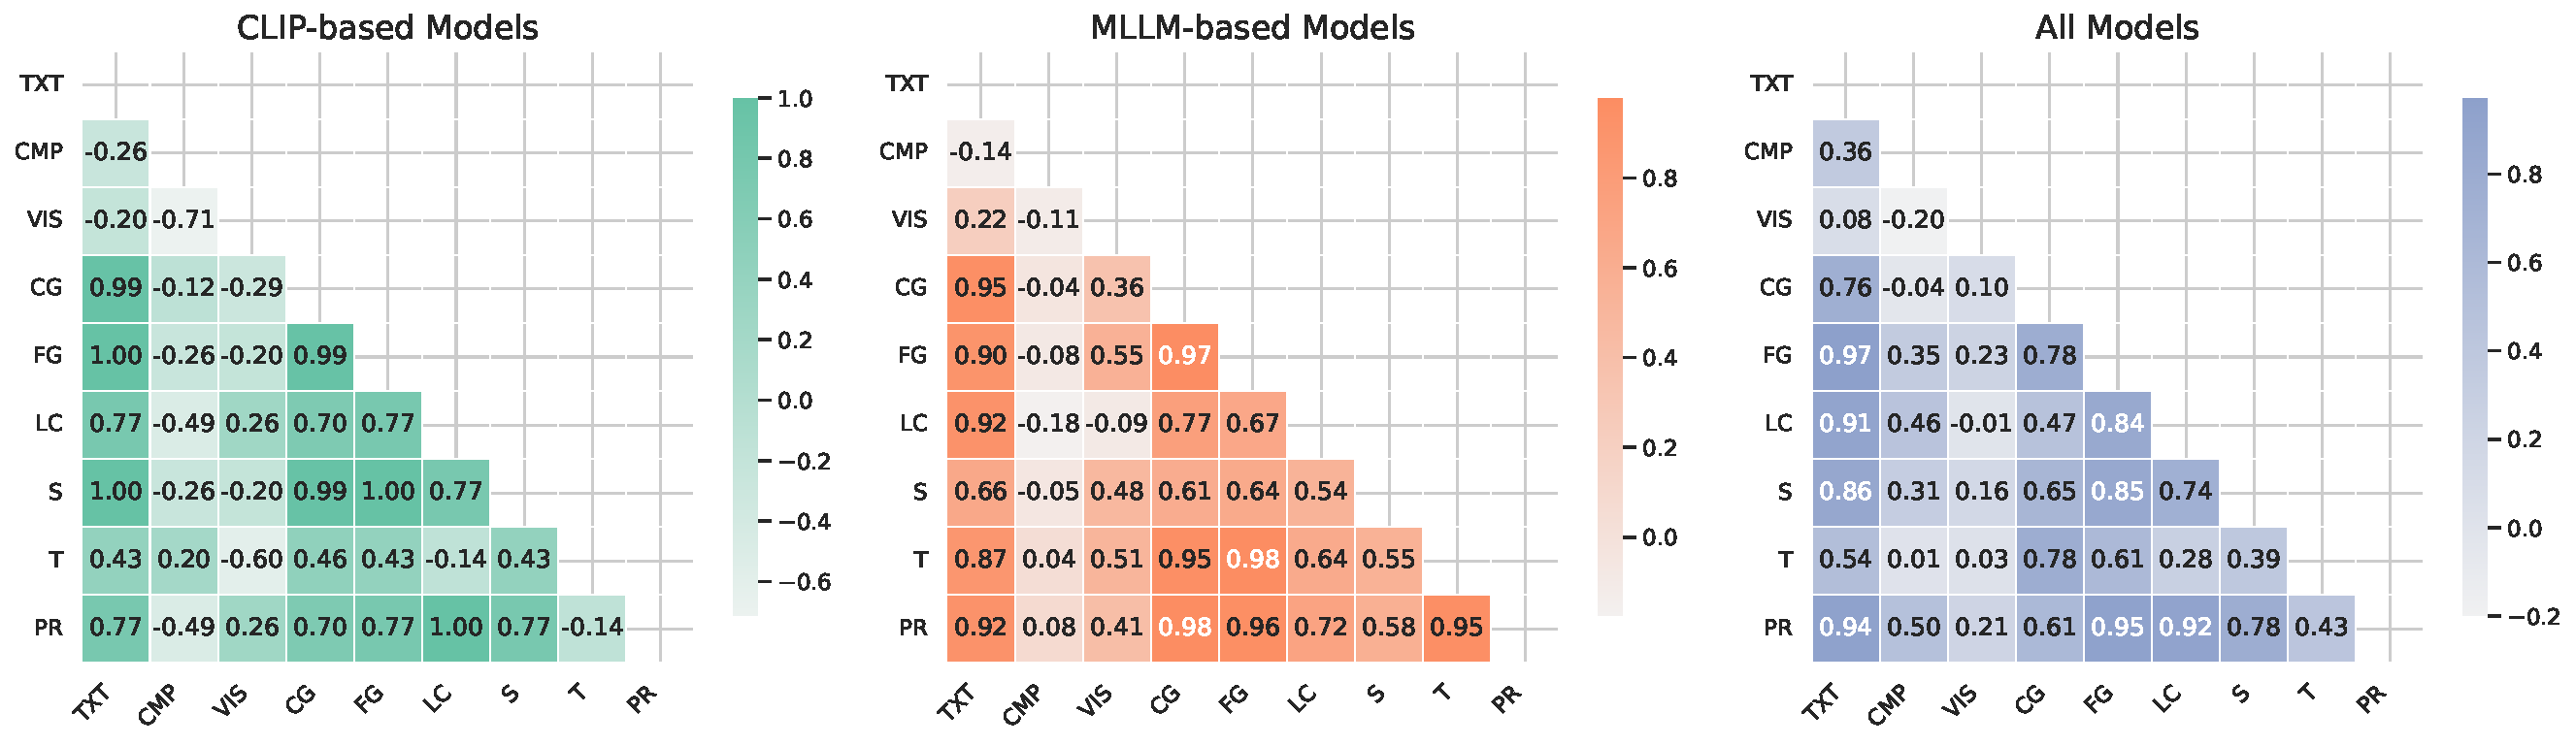
\includegraphics[width=\linewidth]{figures/gve/corr_matrices.pdf}
    \caption{Correlation between dimensional abilities on UVRB for CLIP- and MLLM-based models.}
    \label{gve:fig:corr_ability}
\end{figure}

\begin{figure}[t]
    \centering
    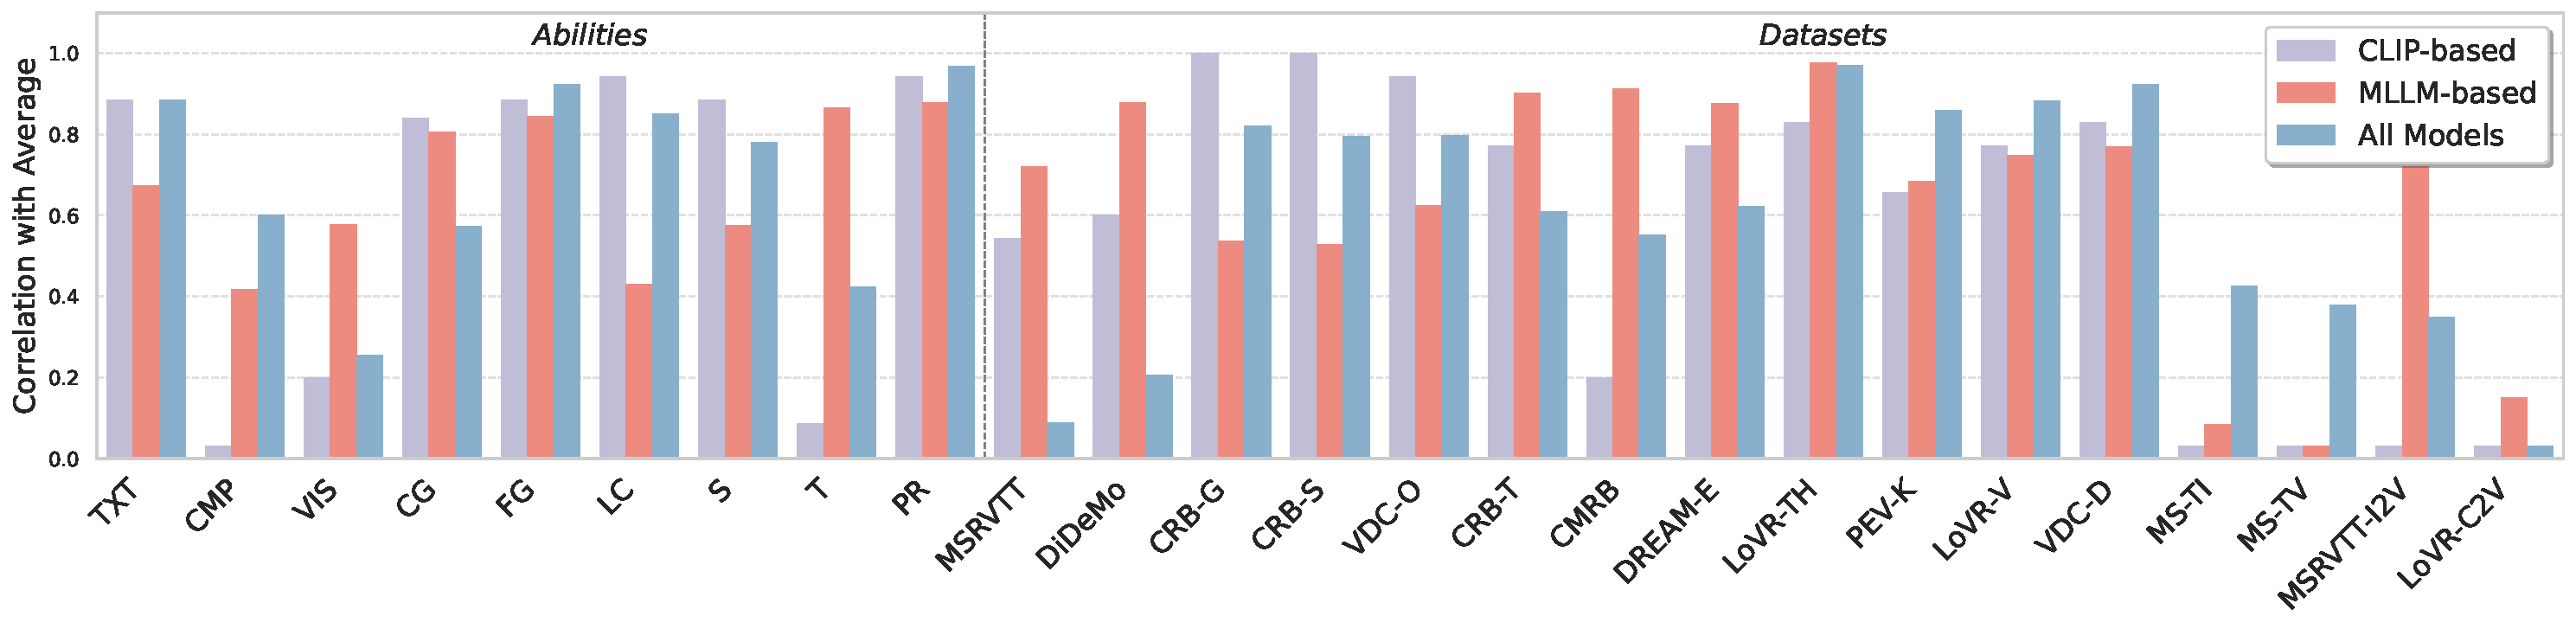
\includegraphics[width=\linewidth]{figures/gve/corr_ability_and_data.pdf}
    \caption{Correlation between averaged performance and individual abilities or datasets on UVRB.}
    \label{gve:fig:corr_task_data}
\end{figure}

\paragraph{Finding 1: Partially Relevant Video Retrieval Better Reflects Universality than Traditional Benchmarks.}
Standard benchmarks such as MSRVTT show a low correlation with average UVR performance ($\rho_{\text{avg}} = 0.58$), suggesting limited representativeness, likely due to overfitting or simplified task design. In contrast, fine-grained (FG), partially relevant (PR), and long-context (LC) retrieval exhibit strong mutual correlations ($\rho \geq 0.90$). More importantly, PR retrieval, although understudied, achieves the highest average correlation with overall performance ($\rho_{\text{avg}} = 0.97$), positioning it as the most reliable proxy for universal capability. We hypothesize this is because successful PR retrieval demands an embedding space that preserves a rich spectrum of information, e.g., from global context to subtle, localized details, rather than collapsing video semantics into a single ``gist''. The ability to maintain this multi-granular semantic richness is a core tenet of universal capability.

\paragraph{Finding 2: Disentangled Spatial and Temporal Representations.}
Models exhibit a marked decoupling between spatial (S) and temporal (T) representation ($\rho = 0.12$). This asymmetry is critical because temporal skills dominate fine-grained understanding ($\rho_{\text{T-FG}} = 0.98$), while spatial skills contribute minimally ($\rho_{\text{S-FG}} = 0.39$). This suggests that current models fail to jointly model \textit{when} and \textit{where}, highlighting the requirements for inductive biases that encourage spatiotemporal integration in video embedding.

\paragraph{Finding 3: Performance Divergence Between CLIP and MLLM-based Models.}
Model failures are architecture-dependent. For example, CLIP-based models are spatially biased ($\rho_{\text{S-CG}} = 0.99$) but temporally weak ($\rho_{\text{T-CG}} = 0.46$), leading to ability trade-offs. Compositional representation inversely correlates with visual accuracy ($\rho_{\text{CMP-VIS}} = -0.71$), and there is a near-zero link between temporal and long-context skills ($\rho_{\text{T-LC}} = -0.14$). In contrast, MLLM-based models demonstrate more balanced and integrated learning: superior semantic matching (PR-CG: MLLM $\rho = 0.98$ vs. CLIP $0.70$) and stronger temporal-long-context coupling ($\rho_{\text{LC-T}} = 0.64$). Therefore, architecture fundamentally shapes the development of capability, and MLLMs have become increasingly popular because of their generalizability in video embedding modeling.

\paragraph{Finding 4: Scaling Has Limited Impact on Visual Perception.}
Parameter scaling improves high-level semantic coherence, but yields negligible gains in low-level visual perception. Notably, the $87$M-parameter \texttt{CLIP4Clip} (VIS: $0.714$) defeats the $8$B-parameter \texttt{Unite-7B} (VIS: $0.702$). Given the weak correlation between visual fidelity and overall retrieval success ($\rho_{\text{AVG-VIS}} = 0.26$), future progress requires targeted improvements in visual grounding.

\FloatBarrier
\subsection{Additional Scaling and Optimization Analyses}

The capability analysis identifies the semantic dimensions that remain difficult. We next examine how training-data scale, inference-time input density, and optimization behavior affect these dimensions. These analyses extend the main comparison by explaining where additional scale helps, where it saturates, and whether the heterogeneous curriculum remains stable during training.


\begin{figure}[t]
    \centering
    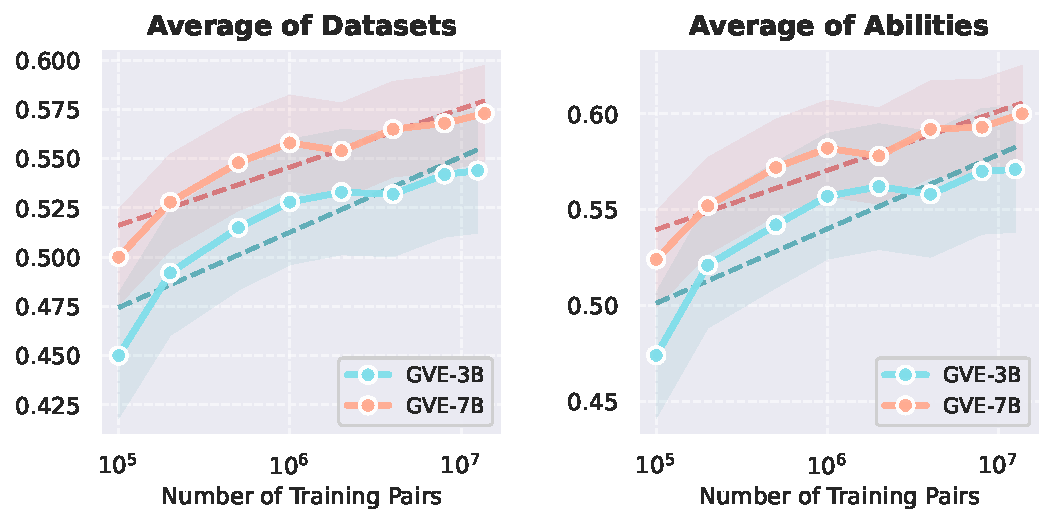
\includegraphics[width=\linewidth]{figures/gve/scaling_avg.pdf}
    \caption{Average performance as a function of training data scale for the GVE series.}
    \label{gve:fig:scaling_avg}
\end{figure}

\subsubsection{Training-Data Scaling}\label{gve:sec:data_scaling}
Figure~\ref{gve:fig:scaling_avg} shows the training-time scaling behavior that performance logarithmically improves with more data, but with diminishing returns.
We quantify scaling efficiency by fitting a logarithmic model $y = a \ln x + b$~($x$: data size, $y$: performance) and report the absolute and relative gain per $10\times$ data increase.
On average across datasets~(abilities), \texttt{GVE-3B} improves by $+7.4\%$~($+7.1\%$) per decade, while \texttt{GVE-7B} gains $+5.4\%$~($+5.4\%$).
While \texttt{GVE-3B} exhibits higher scaling efficiency in relative terms, \texttt{GVE-7B} starts from a higher baseline, suggesting a trade-off between scaling slope and absolute capability.
This result highlights the potential for scaling a more powerful video embedding model with training data at a larger scale.
Figure~\ref{gve:fig:scaling_detail} further decomposes this trend by capability. GVE-3B improves more rapidly on semantic and compositional tasks, including a $14.7\%$ relative gain on CMP and an $11.1\%$ gain on CG per decade of data. GVE-7B shows smaller relative gains on these tasks but benefits more on long-context retrieval, where it improves by $5.4\%$ compared with $3.8\%$ for GVE-3B. This task-dependent pattern suggests that model size affects not only absolute capability but also the scaling profile of different retrieval abilities.

\begin{figure}[t]
    \centering
    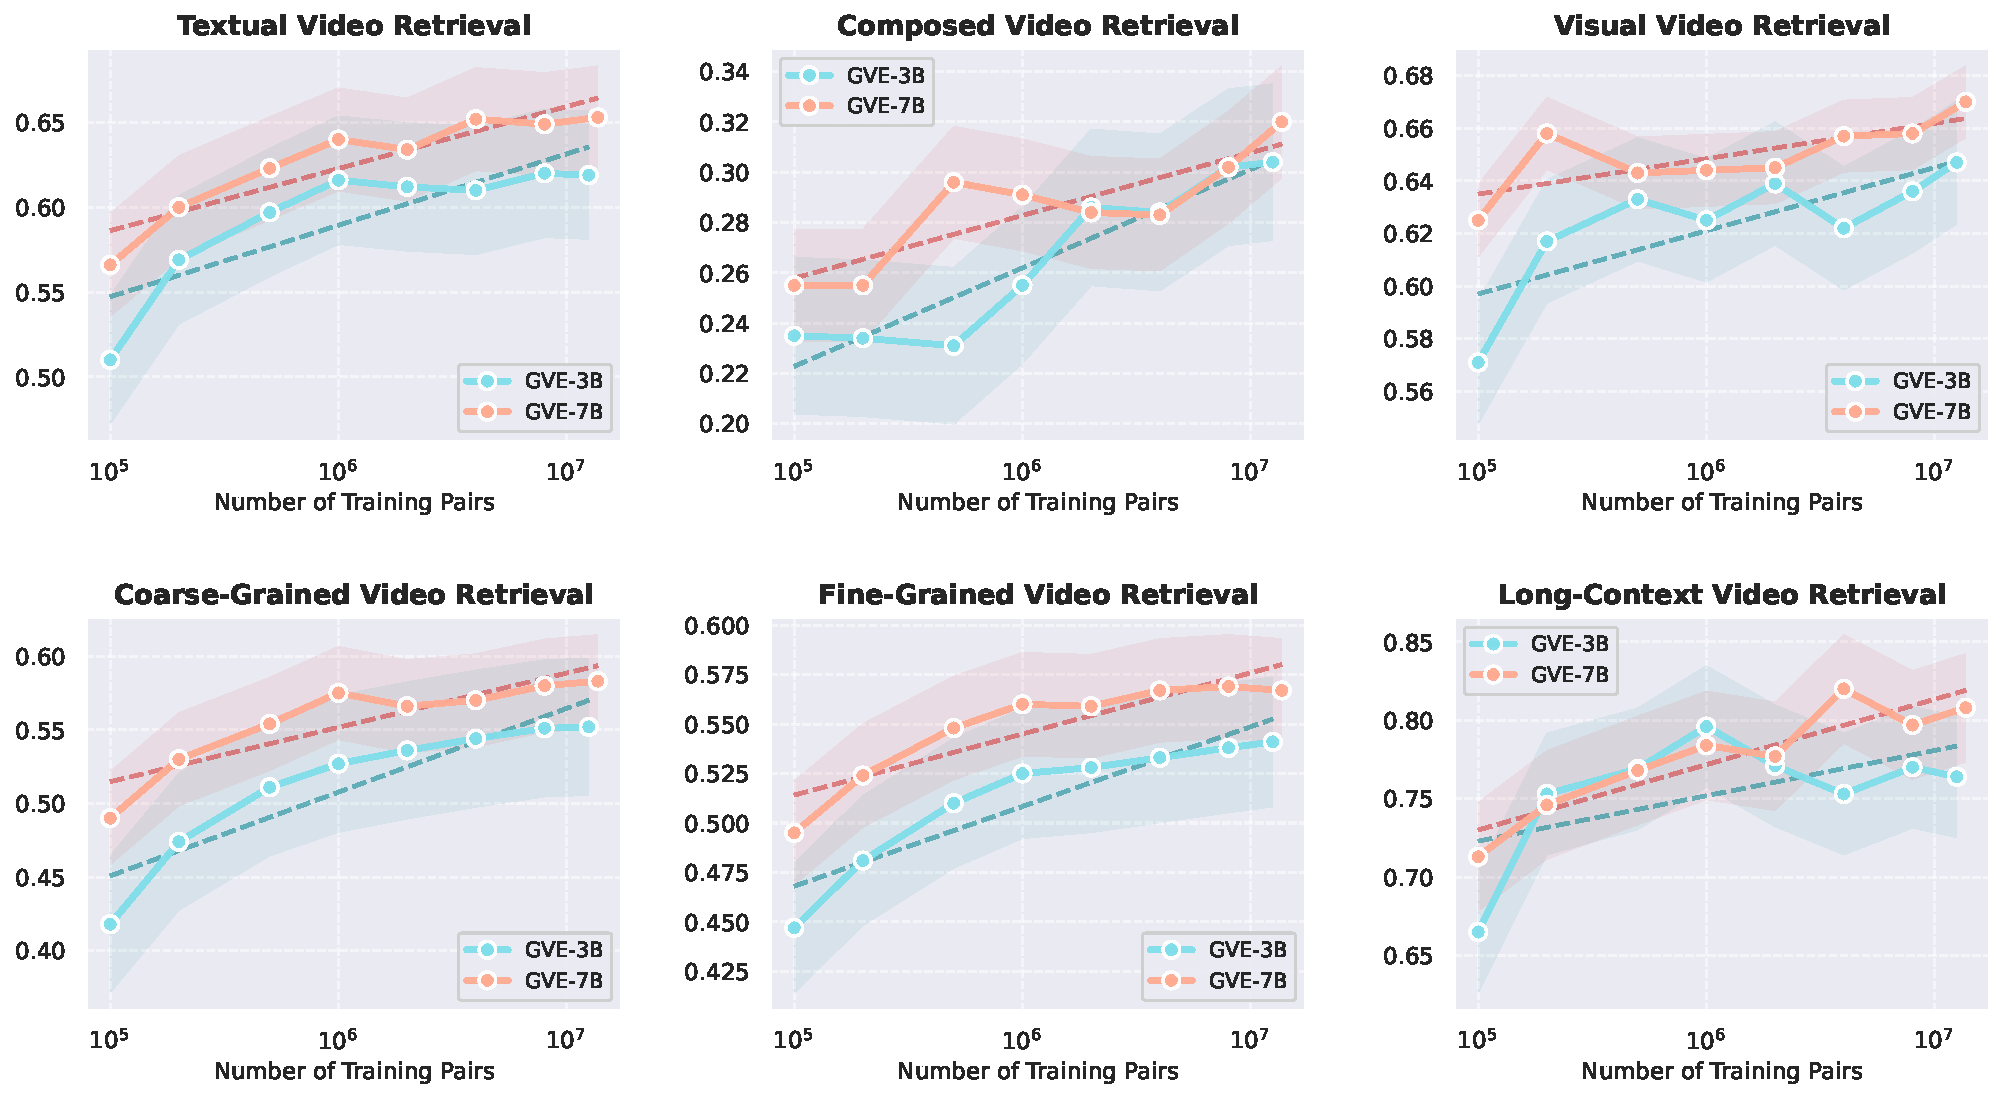
\includegraphics[width=\linewidth]{figures/gve/scaling_detail.pdf}
    \caption{Capability-specific training-data scaling results for GVE-3B and GVE-7B. Shaded bands show $\pm1$ standard deviation, and dashed curves are log-linear fits.}
    \label{gve:fig:scaling_detail}
\end{figure}

\subsubsection{Test-Time Scaling}
We investigate two inference-time parameters for GVE: the number of sampled frames and the maximum number of tokens per frame, which determines the effective spatial resolution. We vary each parameter independently. When the frame count increases from $8$ to $48$, the maximum token count is fixed at $200$. When the token count increases from $200$ to $800$, the frame count is fixed at $8$.

\textit{Temporal scaling.}
As shown in Figure~\ref{gve:fig:scaling_frame}, increasing the number of sampled frames generally improves performance. The largest gains appear in Long-Context retrieval (GVE-3B: $+19.6\%$, GVE-7B: $+12.8\%$), underscoring the value of denser temporal sampling for long-range reasoning. Composed retrieval instead shows a slight degradation, suggesting sensitivity to redundant visual cues from excessive frames. Although GVE-7B consistently outperforms GVE-3B, the average gap across datasets narrows from $0.029$ to $0.024$ as the frame count increases. This indicates that the larger model extracts information more efficiently from sparse inputs.

\textit{Spatial scaling.}
Increasing the token budget yields non-monotonic returns (Figure~\ref{gve:fig:scaling_resolution}). Performance for most tasks peaks around $400$ tokens and then declines. This suggests an optimal level of spatial detail for semantic retrieval. Beyond that point, redundant fine-grained features can dilute the effective semantic signal within the context window. Composed retrieval again deteriorates as the token count increases, reinforcing its sensitivity to input redundancy.

\textit{Implications.}
The results show that temporal scaling provides reliable but diminishing gains, particularly for long-range tasks. Spatial scaling instead exhibits a clear optimum around $400$ tokens, after which additional detail becomes a distraction. The smaller GVE-3B model benefits more from input scaling, whereas GVE-7B shows greater intrinsic efficiency under sparse inputs. These model-specific observations motivate the systematic study of spatiotemporal allocation and density mismatch in Chapter~\ref{ch:spatiotemporal-scaling}.

\begin{figure}[!t]
    \centering
    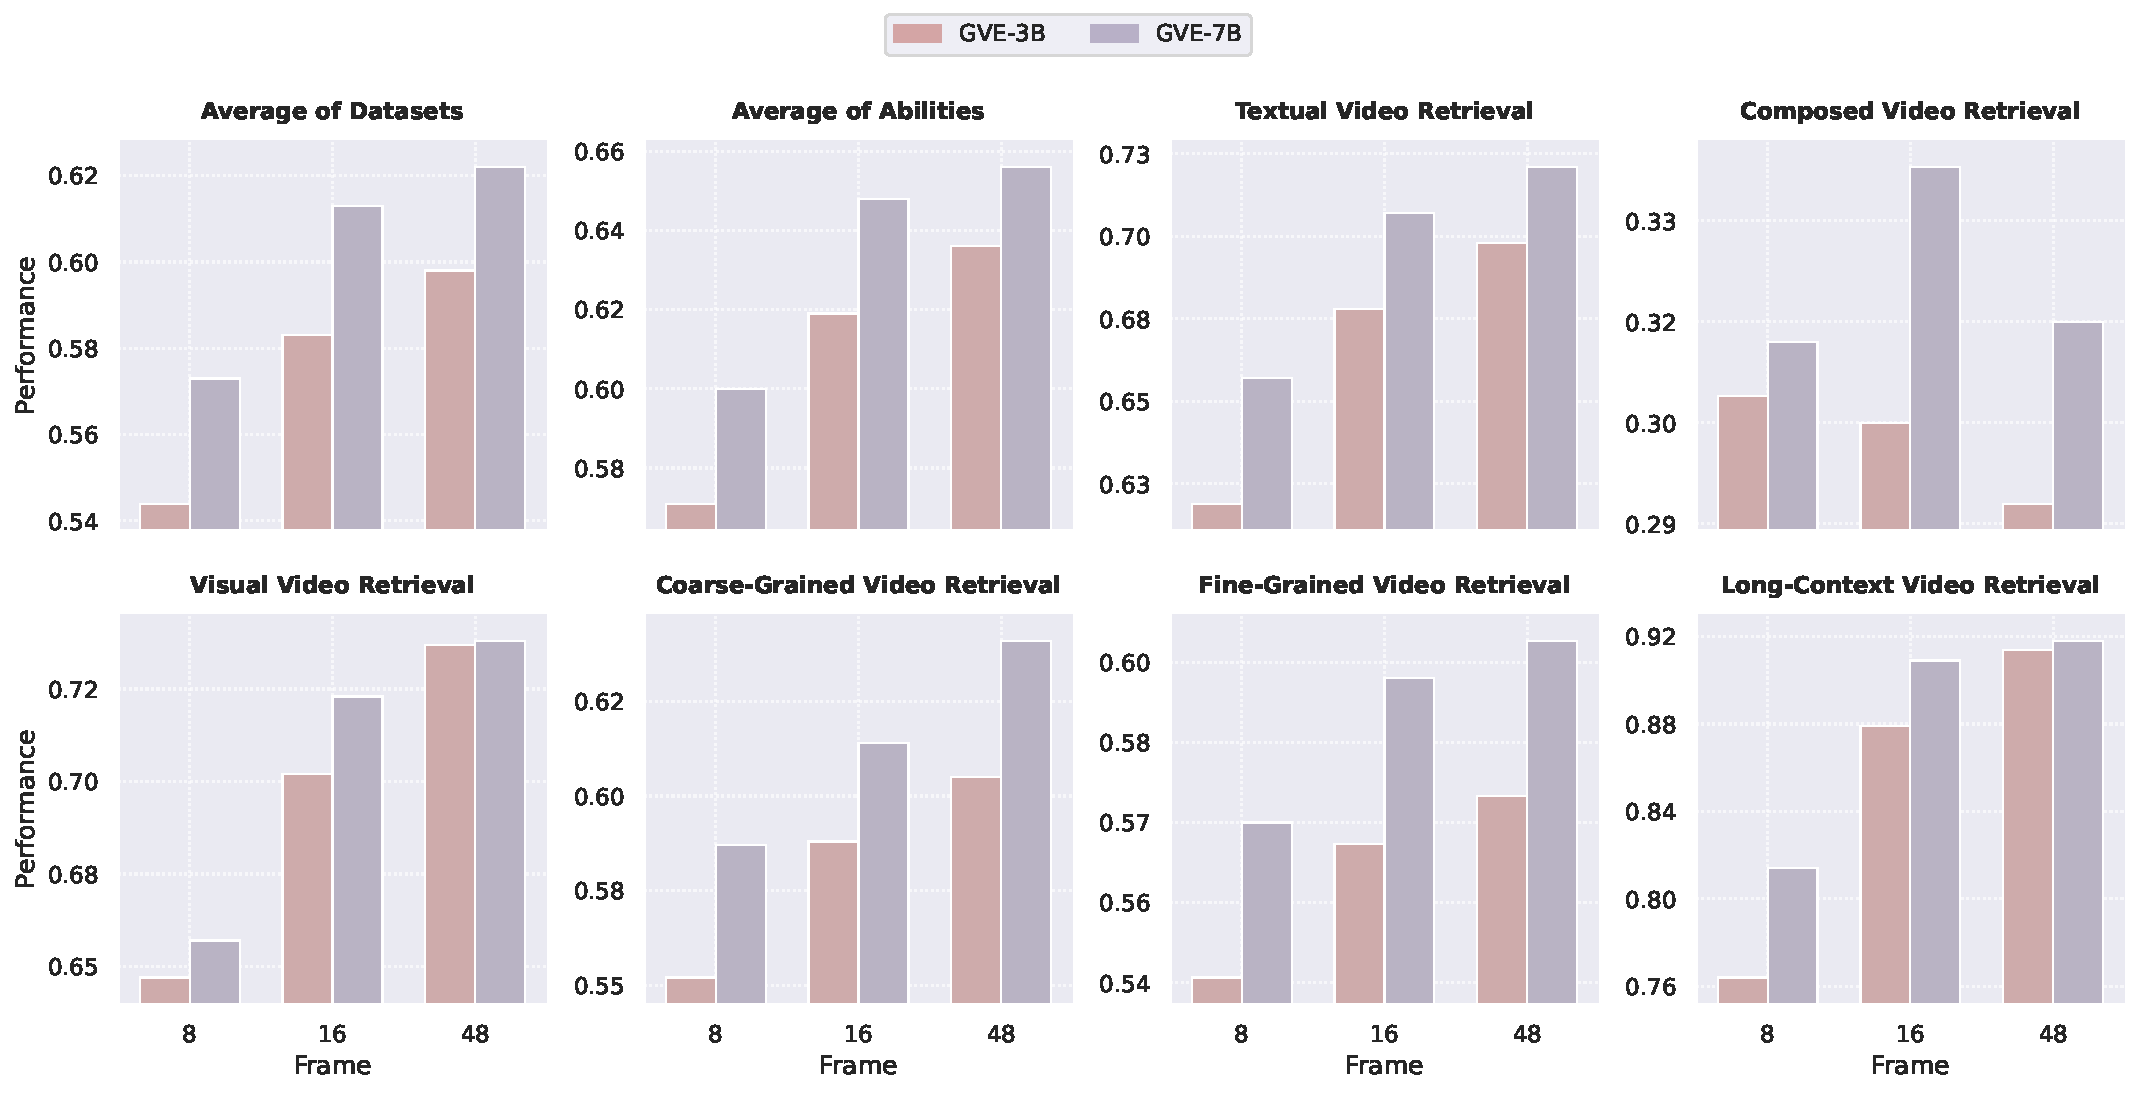
\includegraphics[width=\linewidth]{figures/gve/scaling_frame.pdf}
    \caption{GVE performance as a function of the number of sampled frames at inference time, with the maximum token count fixed at $200$.}
    \label{gve:fig:scaling_frame}

    \vspace{0.5em}
    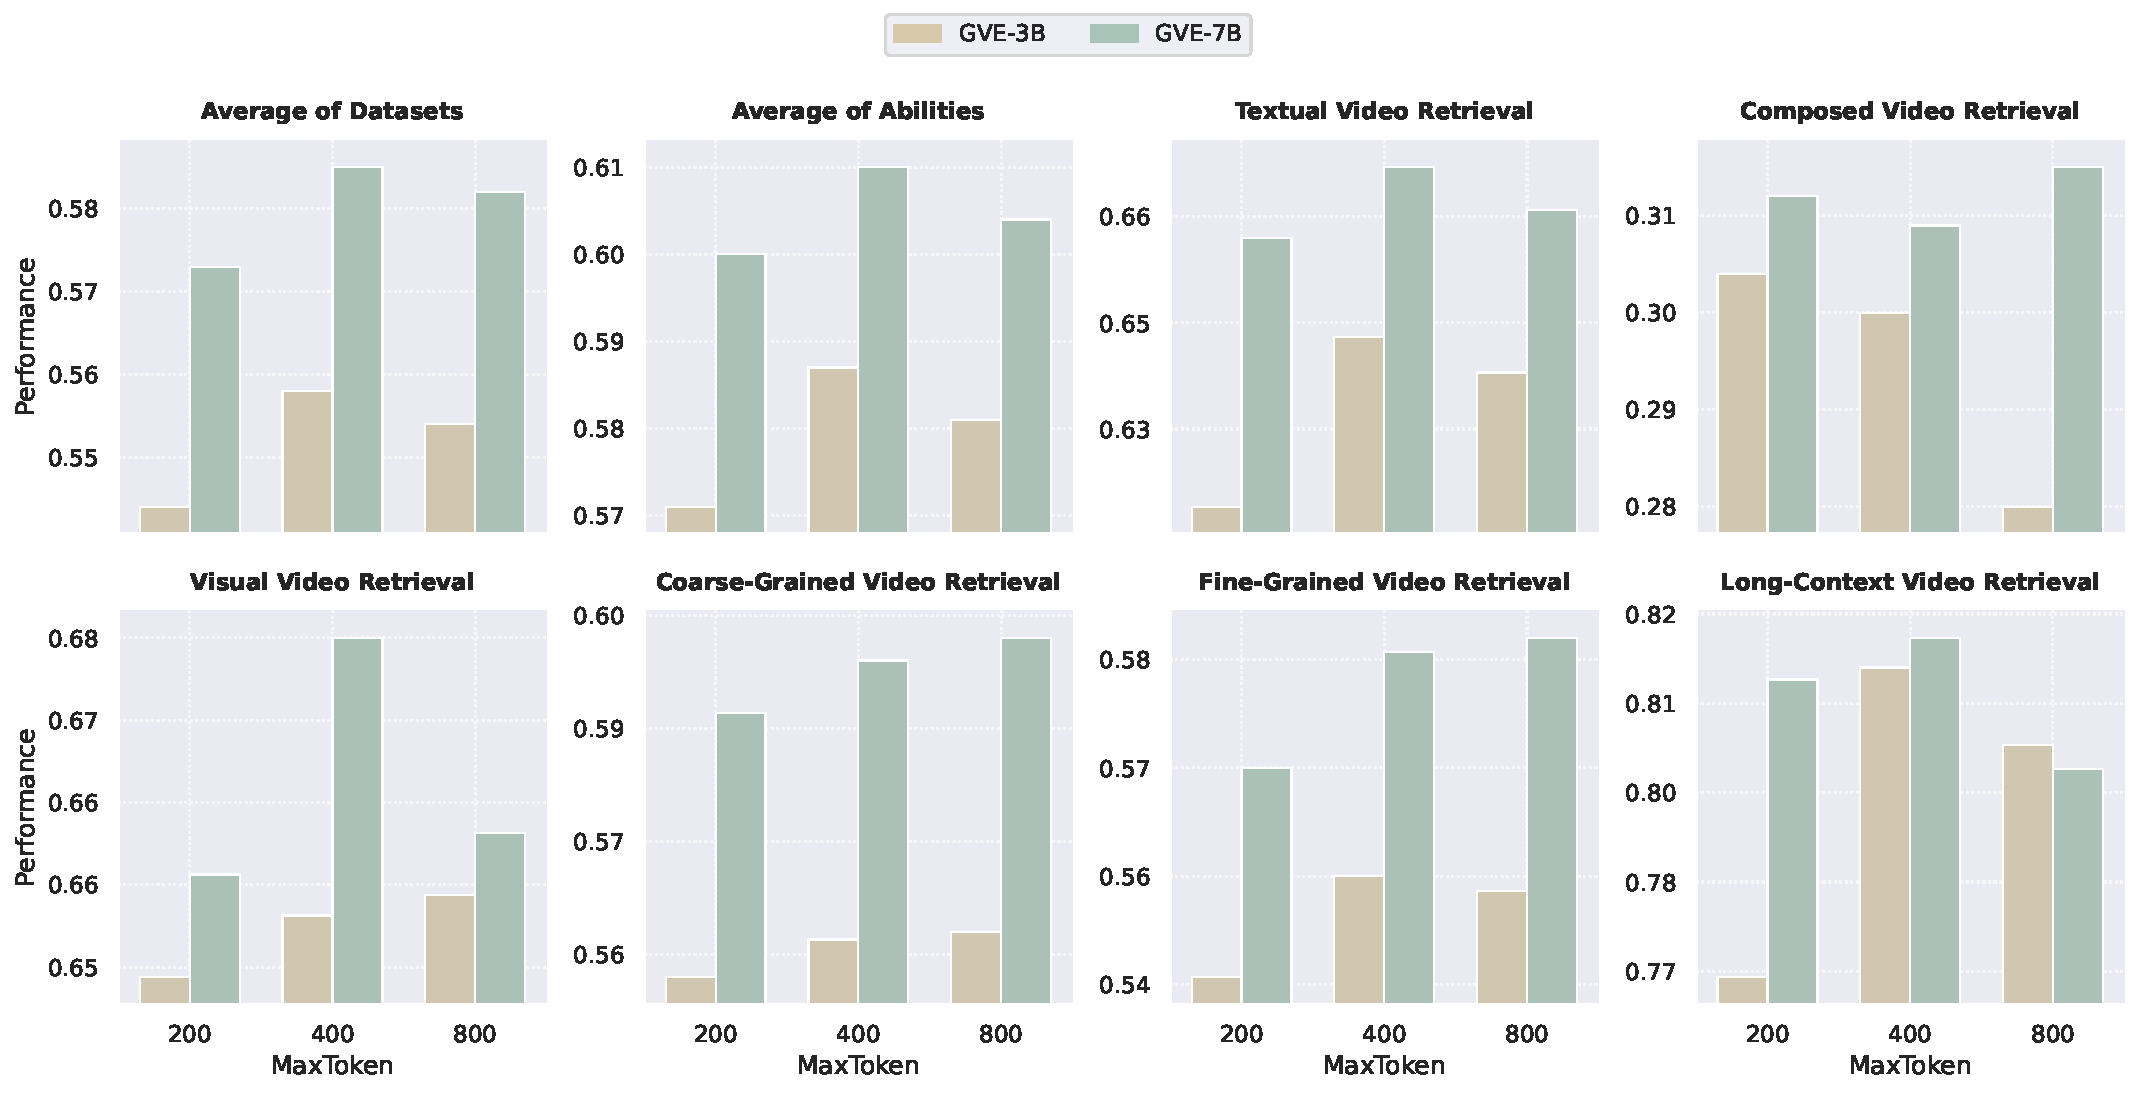
\includegraphics[width=\linewidth]{figures/gve/scaling_resolution.pdf}
    \caption{GVE performance versus the maximum number of tokens per frame, with the frame count fixed at $8$.}
    \label{gve:fig:scaling_resolution}
\end{figure}

\subsubsection{Training Dynamics}
Finally, we inspect optimization stability through four logged quantities: \textit{Training Loss}, \textit{Mean Score}, \textit{Max Negative Gap}, and \textit{Mean Positive Score}. Figure~\ref{gve:fig:training_dynamics} reports the trajectories for GVE-3B and GVE-7B. To reduce the visual influence of isolated outliers, the plots include a $200$-step moving average together with original trajectories subsampled every $100$ steps. Shaded bands indicate $\pm1$ local standard deviation.

\begin{figure}[!t]
    \centering
    \subfloat[GVE-3B.]{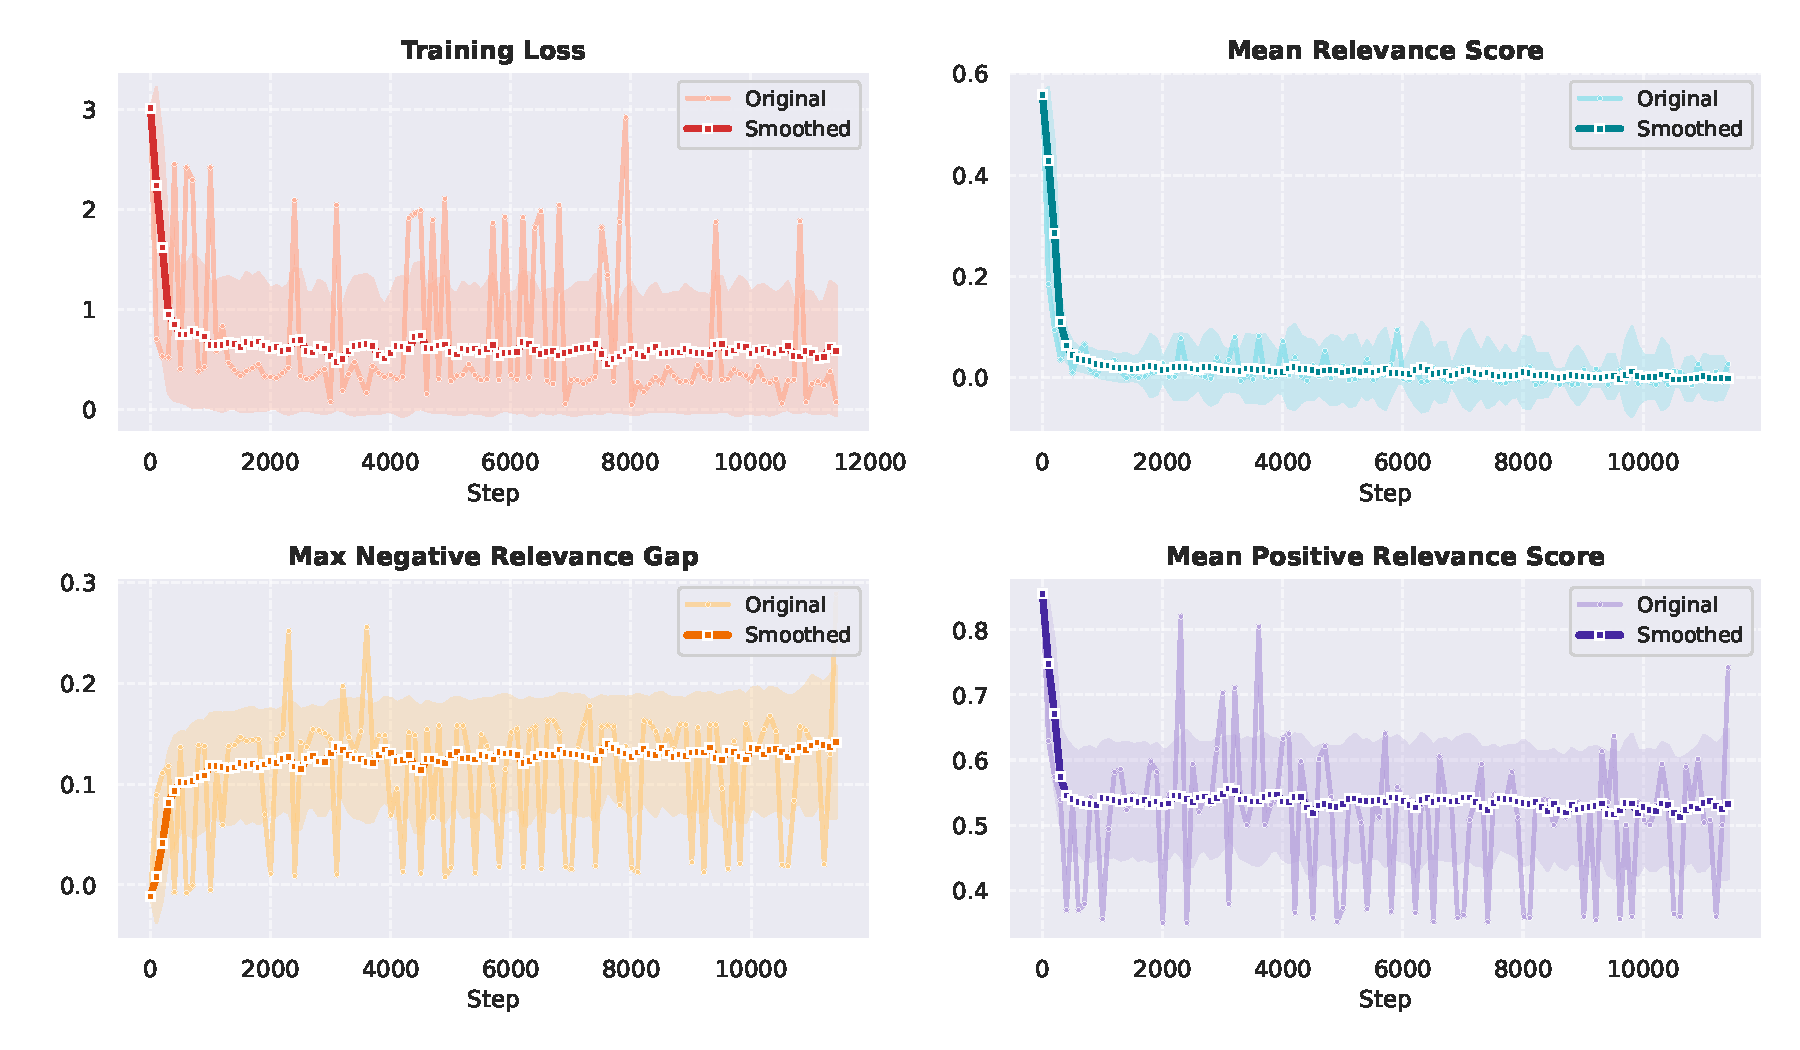
\includegraphics[width=\linewidth]{figures/gve/train_stat-qwen25vl_3b_all_0911.pdf}}\\[-0.5ex]
    \subfloat[GVE-7B.]{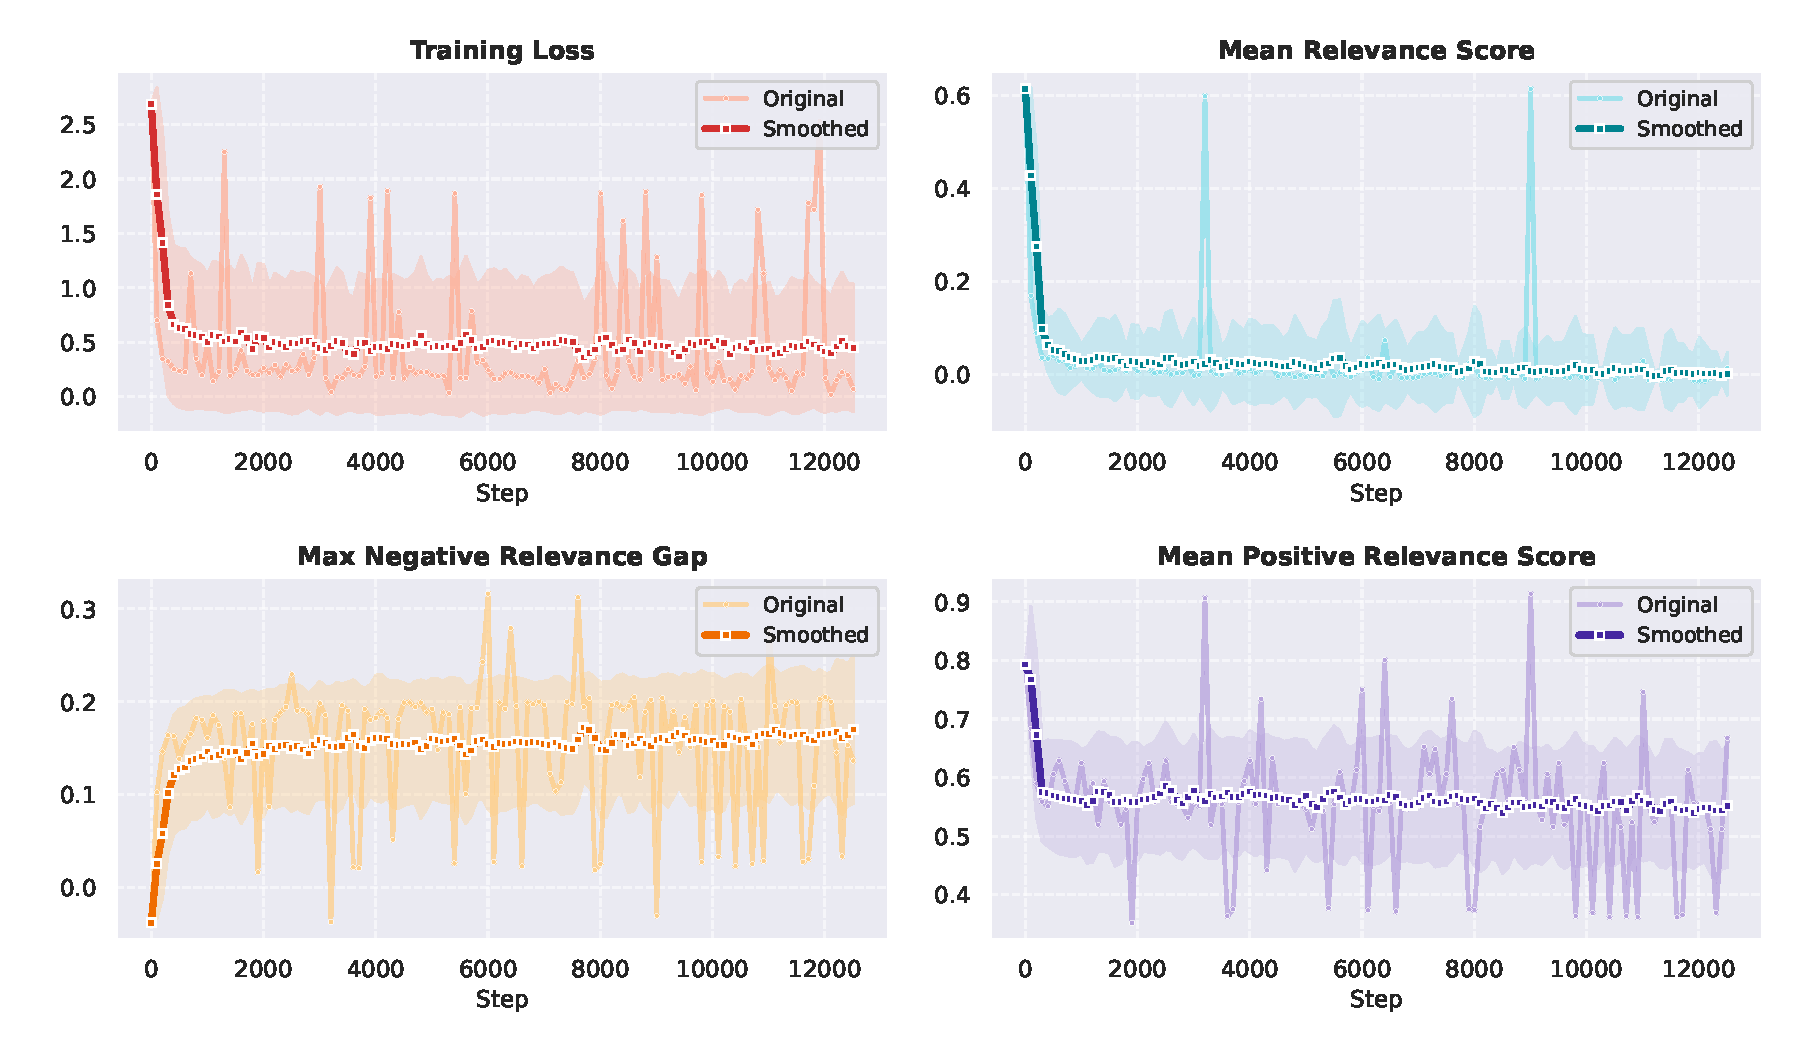
\includegraphics[width=\linewidth]{figures/gve/train_stat-qwen25vl_7b_all_0912.pdf}}
    \caption{Training dynamics of the GVE models across four optimization metrics.}
    \label{gve:fig:training_dynamics}
\end{figure}

\FloatBarrier
\subsection{Zero-Shot Video Classification}

\begingroup\emergencystretch=2em
The preceding experiments evaluate generalization within the UVR capability space. To test whether the learned representation also transfers beyond retrieval, we evaluate GVE on Kinetics-700 (K700)~\cite{carreira2019short}, UCF101~\cite{soomro2012ucf101}, HMDB51~\cite{kuehne2011hmdb}, Something-Something-V2 (SSV2)~\cite{goyal2017something}, and Breakfast~\cite{kuehne2014language}, following MMEB-V2~\cite{meng2025vlm2vec}. Each task is cast as video-to-text retrieval over the complete label set using the standard validation or test split, without training on the target datasets.
\par\endgroup

Table~\ref{gve:tab:video_classification} shows that GVE-7B and InternVideo2-6B attain the highest mean accuracy of $0.526$. GVE-7B also achieves the best UCF101 accuracy and competitive results on the other datasets, indicating that the unified embedding transfers to label-space matching without task-specific adaptation. The lower results on temporally complex datasets such as Breakfast and SSV2 are consistent with the temporal modeling bottleneck identified by the dimensional analysis. The classification results therefore provide an external transfer check while preserving the same zero-shot evaluation principle used throughout the chapter.

\begin{table}[t]
\centering
\caption{Zero-shot video classification accuracy. The highest and second-highest results in each column are bolded and underlined, respectively.}
\label{gve:tab:video_classification}
\begin{tabular}{@{}l|>{\columncolor{gray!15}}c|*{5}{c}@{}}
\toprule
\textbf{Model} & \textbf{AVG} & \textbf{K700} & \textbf{UCF101} & \textbf{HMDB51} & \textbf{SSV2} & \textbf{Breakfast} \\
\midrule
CLIP4Clip       & 0.378 & 0.395 & 0.596 & 0.413 & 0.308 & 0.176 \\
InternVideo2-6B & \textbf{0.526} & \textbf{0.554} & 0.572 & 0.480 & \textbf{0.569} & \textbf{0.453} \\
VLM2Vec-V2      & 0.393 & 0.380 & 0.600 & 0.409 & 0.428 & 0.148 \\
GME-7B          & 0.374 & 0.397 & 0.547 & 0.479 & 0.306 & 0.143 \\
UniME-7B        & 0.306 & 0.388 & 0.377 & 0.407 & 0.190 & 0.166 \\
Unite-7B        & \underline{0.519} & 0.537 & \underline{0.752} & \textbf{0.534} & 0.513 & 0.261 \\
\midrule
GVE-3B          & 0.476 & 0.489 & 0.661 & 0.483 & 0.471 & 0.277 \\
GVE-7B          & \textbf{0.526} & \underline{0.540} & \textbf{0.757} & \underline{0.525} & \underline{0.521} & \underline{0.289} \\
\bottomrule
\end{tabular}
\end{table}

\FloatBarrier
\section{Chapter Summary}

This chapter addressed the semantic-scaling stage of the thesis by asking how one video embedding model can generalize across heterogeneous query formats, domains, and levels of semantic detail. It formulated universal video retrieval and organized 16 public datasets into the UVRB evaluation protocol. The chapter then introduced V-SynFlow and UVRD to supply targeted supervision for underrepresented retrieval capabilities, together with the Modality Pyramid curriculum to stabilize learning across heterogeneous tasks. The main results and ablations showed that both the synthesized data and the curriculum contribute to the performance of GVE under zero-shot evaluation.

The dimensional analysis further showed that conventional benchmarks alone do not adequately represent universal retrieval capability. Partially relevant, fine-grained, and long-context retrieval provide stronger diagnostic signals, while spatial and temporal abilities remain weakly coupled. The scaling, training-dynamics, and video-classification studies clarified how these capabilities respond to additional data, denser inputs, and transfer beyond retrieval. Within the thesis, this chapter establishes broad semantic coverage as the first requirement for scalable video retrieval. It also exposes a remaining limitation: a semantically general representation can only use evidence that is present in its sampled input. This limitation motivates the observational-scaling study in Chapter~\ref{ch:spatiotemporal-scaling}.
